%%%%%%%%%%%%%%%%%%%%%%%%%%%%%% -*- Mode: Latex -*- %%%%%%%%%%%%%%%%%%%%%%%%%%%%
%% 05-01-appendix.tex -- 
%% Author          : Aaron A. Kagawa
%% Created On      : Tue Sept 21 12:04:50 2004
%% Last Modified By: Aaron Kagawa
%% Last Modified On: Tue Jun 14 21:17:03 2005
%% Status          : Unknown
%% RCS: $Id: 04-appendix.tex,v 1.3 2000/03/17 21:28:36 rbrewer Exp $
%%%%%%%%%%%%%%%%%%%%%%%%%%%%%%%%%%%%%%%%%%%%%%%%%%%%%%%%%%%%%%%%%%%%%%%%%%%%%%%
%%   Copyright (C) 1998 Robert Brewer
%%%%%%%%%%%%%%%%%%%%%%%%%%%%%%%%%%%%%%%%%%%%%%%%%%%%%%%%%%%%%%%%%%%%%%%%%%%%%%%
%% 

\appendix

\chapter{Consent Form}
\label{appendix:consent}
\begin{figure}[!htbp]
  \centering
  \includegraphics[width=1.0\textwidth]{figs/ConsentForm_shrunk.eps}
  \caption{Consent Form}
  \label{fig:consent}
\end{figure}
%%%%%%%%%%%%%%%%%%%%%%%%%%%%%%%%%%%%%%%%%%%%%%%%%%%%%%%%%%%%%%%%%%%%%%%%%%%%%%%

\chapter{Pre-Selection Questionnaire}
\label{appendix:pre-selection-questionnaire}

\begin{figure}[htbp]
  \centering
  \includegraphics[width=1.0\textwidth]{figs/Questionnaire-Pre-shrunk_1.eps}
  \caption{Pre-Selection Questionnaire - Part 1}
  \label{fig:questionnaire-pre1}
\end{figure}

\begin{figure}[htbp]
  \centering
  \includegraphics[width=1.0\textwidth]{figs/Questionnaire-Pre-shrunk_2.eps}
  \caption{Pre-Selection Questionnaire - Part 2}
  \label{fig:questionnaire-pre2}
\end{figure}

\begin{figure}[htbp]
  \centering
  \includegraphics[width=1.0\textwidth]{figs/Questionnaire-Pre-shrunk_3.eps}
  \caption{Pre-Selection Questionnaire - Part 3}
  \label{fig:questionnaire-pre3}
\end{figure}

\begin{figure}[htbp]
  \centering
  \includegraphics[width=1.0\textwidth]{figs/Questionnaire-Pre-shrunk_4.eps}
  \caption{Pre-Selection Questionnaire - Part 4}
  \label{fig:questionnaire-pre4}
\end{figure}
%%%%%%%%%%%%%%%%%%%%%%%%%%%%%%%%%%%%%%%%%%%%%%%%%%%%%%%%%%%%%%%%%%%%%%%%%%%%%%%


\chapter{Post-Inspection Questionnaire}
\label{appendix:post-inspection-questionnaire}

\begin{figure}[!htbp]
  \centering
  \includegraphics[width=1.0\textwidth]{figs/Questionnaire-Post-Inspection-shrunk.eps}
  \caption{Post-Inspection Questionnaire}
  \label{fig:questionnaire-post-inspection}
\end{figure}
%%%%%%%%%%%%%%%%%%%%%%%%%%%%%%%%%%%%%%%%%%%%%%%%%%%%%%%%%%%%%%%%%%%%%%%%%%%%%%%


\chapter{Pre-Selection-Questionnaire Results}
\label{appendix:chapter:pre-selection-questionnaire-results}
This section contains the results from the Pre-Selection-Questionnaire.
Sections \ref{appendix:section:question1} and \ref{appendix:section:question2} contains
the results from the general questions about CSDL's inspection process.
Section \ref{appendix:section:question3} to Section \ref{appendix:section:question6}
contains the results from the questions about the developers' document
selection method. Section \ref{appendix:section:question7} to Section
\ref{appendix:section:question9} contains the results from the developers'
subjective rankings of three separate sets of packages.

\clearpage
\section{Question 1}
\label{appendix:section:question1}
\noindent \textbf{Question 1.} Inspections are an important part of the CSDL
  development process. (Choose One)

(1) Strongly Disagree (2) Disagree (3) Neutral (4) Agree (5) Strongly Agree

\begin{table}[!h]
  \begin{center}
    \caption{Question 1 Responses}
    \label{tab:pre-selection-questionnaire-results-1}
    \begin{tabular}{|p{5.0cm}|p{8.0cm}|} \hline
{\bf Participant} & {\bf Response} \\ \hline
1 & Strongly Agree \\ \hline
2 & Strongly Agree \\ \hline
3 & Strongly Agree \\ \hline
4 & Agree \\ \hline
5 & Strongly Agree \\ \hline
6 & Agree \\ \hline
    \end{tabular}
  \end{center}
\end{table}

\begin{figure}[htb]
  \centering
  \includegraphics[width=1.0\textwidth]{figs/Results/pre-selection-questionnaire-1.eps}
  \caption{Question 1 Responses}
  \label{fig:pre-selection-questionnaire-results-1}
\end{figure}


\clearpage
\section{Question 2}
\label{appendix:section:question2}
\noindent \textbf{Question 2.} The most important goal of the CSDL
inspection process is to remove defects. (Choose One)

(1) Strongly Disagree (2) Disagree (3) Neutral (4) Agree (5) Strongly Agree

\begin{table}[!h]
  \begin{center}
    \caption{Question 2 Responses}
    \label{tab:pre-selection-questionnaire-results-2}
    \begin{tabular}{|p{5.0cm}|p{8.0cm}|} \hline
{\bf Participant} & {\bf Response} \\ \hline
1 & Neutral \\ \hline
2 & Agree \\ \hline
3 & Neutral \\ \hline
4 & Disagree \\ \hline
5 & Agree \\ \hline
6 & Neutral \\ \hline
    \end{tabular}
  \end{center}
\end{table}

\begin{figure}[htb]
  \centering
  \includegraphics[width=1.0\textwidth]{figs/Results/pre-selection-questionnaire-2.eps}
  \caption{Question 2 Responses}
  \label{fig:pre-selection-questionnaire-results-2}
\end{figure}

%%Part 2 - Developers Selection Method

\clearpage
\section{Question 3}
\label{appendix:section:question3}
\noindent \textbf{Question 3.} Which of the following would most likely
contain the most critical defects (Choose all that apply)

(1) Newly created code \newline
\indent (2) Code that has no (or very few) unit tests \newline
\indent (3) Code that has low coverage \newline
\indent (4) Code that was developed by a new developer \newline
\indent (5) Code that only one developer has worked on \newline
\indent (6) Code that has a large number of dependencies \newline
\indent (7) Old code \newline
\indent (8) Other:  \newline

\begin{table}[!h]
  \begin{center}
    \caption{Question 3 Responses}
    \label{tab:pre-selection-questionnaire-results-3}
    \begin{tabular}{|p{3.0cm}|p{10.0cm}|} \hline
{\bf Participant} & {\bf Response} \\ \hline
1 & (1), (2), (3), (4), (5) \\ \hline
2 & (1), (2), (3), (4) \\ \hline
3 & (1), (4), (6) \\ \hline
4 & Other: Strongly Refactored Code \\ \hline
5 & (4) \\ \hline
6 & (4) \\ \hline
    \end{tabular}
  \end{center}
\end{table}

\begin{figure}[htb]
  \centering
  \includegraphics[width=1.0\textwidth]{figs/Results/pre-selection-questionnaire-3.eps}
  \caption{Question 3 Responses}
  \label{fig:pre-selection-questionnaire-results-3}
\end{figure}


\clearpage
\section{Question 4}
\label{appendix:section:question4}
\noindent \textbf{Question 4.} When I request an inspection, I generally
volunteer code that is: (Choose all that apply)

(1) Newly created code \newline
\indent (2) Code that has low coverage \newline
\indent (3) Code that no has seen before \newline
\indent (4) Code that has no unit tests \newline
\indent (5) Old code \newline
\indent (6) Other: \newline

\begin{table}[!h]
  \begin{center}
    \caption{Question 4 Responses}
    \label{tab:pre-selection-questionnaire-results-4}
    \begin{tabular}{|p{3.0cm}|p{10.0cm}|} \hline
{\bf Participant} & {\bf Response} \\ \hline
1 & (1), (3), (5) \\ \hline
2 & (1), (3) \\ \hline
3 & (1), (3) \\ \hline
4 & Other: Fulfills a critical mission; is to be used by others \\ \hline
5 & (3) \\ \hline
6 & Other: Code I have no confidence in. Code that I feel is badly designed 
\\ \hline
    \end{tabular}
  \end{center}
\end{table}

\begin{figure}[htb]
  \centering
  \includegraphics[width=1.0\textwidth]{figs/Results/pre-selection-questionnaire-4.eps}
  \caption{Question 4 Responses}
  \label{fig:pre-selection-questionnaire-results-4}
\end{figure}


\clearpage
\section{Question 5}
\label{appendix:section:question5}
\noindent \textbf{Question 5.} When I request an inspection, I use
Hackystat to help me pick a piece of code to inspect? (Choose one)

(1) Strongly Disagree (2) Disagree (3) Neutral (4) Agree (5) Strongly Agree

\begin{table}[!h]
  \begin{center}
    \caption{Question 5 Responses}
    \label{tab:pre-selection-questionnaire-results-5}
    \begin{tabular}{|p{5.0cm}|p{8.0cm}|} \hline
{\bf Participant} & {\bf Response} \\ \hline
1 & Disagree \\ \hline
2 & Disagree \\ \hline
3 & Disagree \\ \hline
4 & Disagree \\ \hline
5 & Disagree \\ \hline
6 & Disagree \\ \hline
    \end{tabular}
  \end{center}
\end{table}

\begin{figure}[htb]
  \centering
  \includegraphics[width=1.0\textwidth]{figs/Results/pre-selection-questionnaire-5.eps}
  \caption{Question 5 Responses}
  \label{fig:pre-selection-questionnaire-results-5}
\end{figure}


\clearpage
\section{Question 6}
\label{appendix:section:question6}
\noindent \textbf{Question 6.} Inspection should only occur on newly
created code. Old code that has already been released does not need to be
inspected. (Choose one)

(1) Strongly Disagree (2) Disagree (3) Neutral (4) Agree (5) Strongly Agree

\begin{table}[!h]
  \begin{center}
    \caption{Question 6 Responses}
    \label{tab:pre-selection-questionnaire-results-6}
    \begin{tabular}{|p{5.0cm}|p{8.0cm}|} \hline
{\bf Participant} & {\bf Response} \\ \hline
1 & Strongly Disagree \\ \hline
2 & Agree \\ \hline
3 & Disagree \\ \hline
4 & Disagree \\ \hline
5 & Neutral \\ \hline
6 & Neutral \\ \hline
    \end{tabular}
  \end{center}
\end{table}

\begin{figure}[htb]
  \centering
  \includegraphics[width=1.0\textwidth]{figs/Results/pre-selection-questionnaire-6.eps}
  \caption{Question 6 Responses}
  \label{fig:pre-selection-questionnaire-results-6}
\end{figure}

%%Part 3 - Developer Ranking

\clearpage
\section{Question 7}
\label{appendix:section:question7}
\noindent \textbf{Question 7.} Please provide a numerical ranking of the
packages provided that represent what packages you believe should be
inspected. Enter your own subjective rankings. Please use values from 1
through N (N denotes the number of packages in the developers list of
packages) and do not use one number twice.

\subsection{hackyReview}
The response to this question contains two results. First, a developer
ranking, which is provided in Table
\ref{tab:hackyReview-developer-ranking}. Second, a PRI ranking, which is
provided in the Figure \ref{fig:inspection8-hackyReview-ranking}.
Furthermore, the results of the developer rankings were used to help aid
the developer in selecting a package for inspection. Therefore, for
Inspection 8, the packages org.hackystat.stdext.analysis.stream and
org.hackystat.stdext.analysis.cache were selected.

In this particular case, the developer ranking and PRI ranking agreed that 
those two packages were MINI packages, relative to other packages in the
same module.


\begin{table}[!h]
  \begin{center}
    \caption{hackyReview Developer Ranking}
    \label{tab:hackyReview-developer-ranking}
    \begin{tabular}{|p{1.5cm}|p{11.5cm}|} \hline
{\bf Ranking} & {\bf Package} \\ \hline
1 & org.hackystat.app.review.analysis.stream \\ \hline
2 & org.hackystat.app.review.analysis.cache \\ \hline
3 & org.hackystat.app.review.analysis \\ \hline
4 & org.hackystat.app.review.analysis.comparison \\ \hline
5 & org.hackystat.app.review.analysis.summary \\ \hline
6 & org.hackystat.app.review.issue.reducer \\ \hline
7 & org.hackystat.app.review.activity.reducer \\ \hline
8 & org.hackystat.app.review.issue.dailyproject \\ \hline
9 & org.hackystat.app.review.activity.dailyproject \\ \hline
10 & org.hackystat.app.review.issue.dailyanalysis \\ \hline
11 & org.hackystat.app.review.activity.dailyanalysis \\ \hline
12 & org.hackystat.app.review.issue.std \\ \hline
13 & org.hackystat.app.review.activity.std \\ \hline
    \end{tabular}
  \end{center}
\end{table}

\begin{figure}[!h]
  \centering
  \caption{hackyReview PRI Ranking - Inspection 8}
  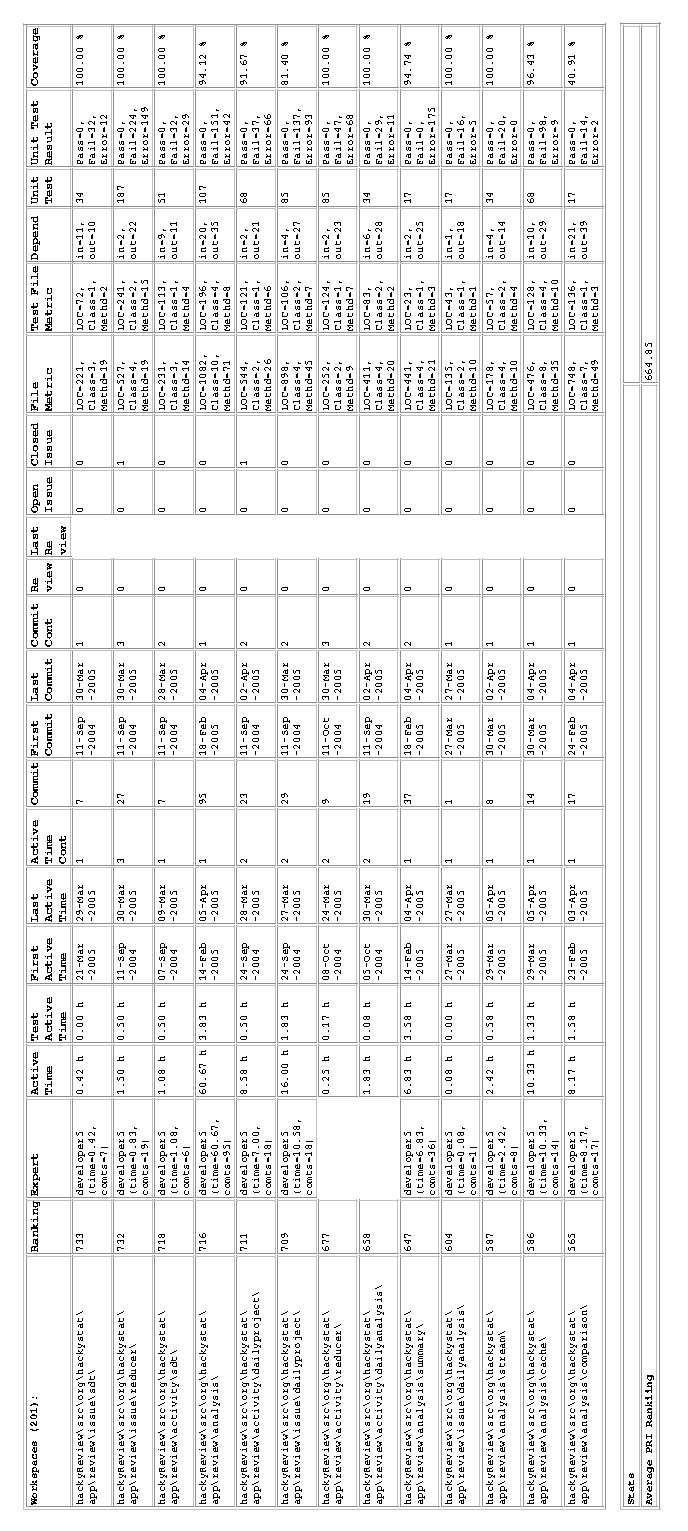
\includegraphics[totalheight=1.0\textheight]{figs/Results/8_2005-04-05-hackyReview-printable.eps}
  \label{fig:inspection8-hackyReview-ranking}
\end{figure}

\clearpage
\subsection{hackyIssue}
The response to this question contains two results. First, a developer
ranking, which is provided in Table \ref{tab:hackyIssue-developer-ranking}.
Second, a PRI ranking, which is provided in the Figure
\ref{fig:inspection9-hackyIssue-ranking}.  Furthermore, the results of the
developer rankings were used to help aid the developer in selecting a
package for inspection. Therefore, for Inspection 9, the package
org.hackystat.stdext.issue.reducer was selected.

In this particular case, the developer ranking and PRI ranking agreed that 
the package was a MINI package, relative to other packages in the
same module.

\begin{table}[!h]
  \begin{center}
    \caption{hackyIssue Developer Ranking}
    \label{tab:hackyIssue-developer-ranking}
    \begin{tabular}{|p{1.5cm}|p{11.5cm}|} \hline
{\bf Ranking} & {\bf Package} \\ \hline
1 & org.hackystat.stdext.issue.reducer \\ \hline
2 & org.hackystat.stdext.issue.dailyproject \\ \hline
3 & org.hackystat.stdext.issue.analysis.issueprojectdetails \\ \hline
4 & org.hackystat.stdext.issue.sdt \\ \hline
    \end{tabular}
  \end{center}
\end{table}

\begin{figure}[!h]
  \centering
  \caption{hackyIssue PRI Ranking - Inspection 9}
  \includegraphics[totalheight=1.0\textheight]{figs/Results/9_2005-04-10-hackyIssue-printable.eps}
  \label{fig:inspection9-hackyIssue-ranking}
\end{figure}

\clearpage
\subsection{hackyCGQM}
The response to this question contains two results. First, a developer
ranking, which is provided in Table
\ref{tab:hackyCGQM-developer-ranking}. Second, a PRI ranking, which is
provided in the Figure \ref{fig:inspection11-hackyCGQM-ranking}.
Furthermore, the results of the developer rankings were used to help aid
the developer in selecting packages for inspection. Therefore, for
Inspection 11, the packages org.hackystat.app.cgqm.interfaces.executables,
org.hackystat.app.cgqm.interfaces.results, and
org.hackystat.app.cgqm.implementations.executables were selected.

In this particular case, the developer ranking and PRI ranking disagreed
that the packages were MINI packages, relative to other packages in the
same module. However, because only one inspection was conducted in this
module, it is not known whether the developer rankings or PRI rankings were
incorrect.

\begin{table}[!h]
  \begin{center}
    \caption{hackyCGQM Developer Ranking}
    \label{tab:hackyCGQM-developer-ranking}
    \begin{tabular}{|p{1.5cm}|p{11.5cm}|} \hline
{\bf Ranking} & {\bf Package} \\ \hline
1 & org.hackystat.app.cgqm.interfaces.executables \\ \hline
2 & org.hackystat.app.cgqm.interfaces.results \\ \hline
3 & org.hackystat.app.cgqm.implementation.executables \\ \hline
4 & org.hackystat.app.cgqm.implementation.results \\ \hline
5 & org.hackystat.app.cgqm.common.classloaders \\ \hline
6 & org.hackystat.app.cgqm.utils \\ \hline
6 & org.hackystat.app.cgqm.datamodel.cgqm\\ \hline
8 & org.hackystat.app.cgqm.datamodels.cgqm.goals \\ \hline
9 & org.hackystat.app.cgqm.datamodels.cgqm.metric \\ \hline
10 & org.hackystat.app.cgqm.datamodels.cgqm.question \\ \hline
11 & org.hackystat.app.cgqm.manager \\ \hline
12 & org.hackystat.app.cgqm.telemetry.reducer \\ \hline
13 & org.hackystat.app.cgqm.testbase \\ \hline
14 & org.hackystat.app.cgqm.utils.freemarker \\ \hline
15 & org.hackystat.app.cgqm.webinterface \\ \hline
16 & org.hackystat.app.cgqm.webinterface.selector \\ \hline
17 & org.hackystat.app.cgqm.datamodels.cgqm.common \\ \hline
18 & org.hackystat.app.cgqm.datamodel.cgqm.goal.goalDimension \\ \hline
19 & org.hackystat.app.cgqm.datamodel.cgqm.goal.sheetComponents \\ \hline
20 & org.hackystat.app.cgqm.common.jiBx \\ \hline
21 & org.hackystat.app.cgqm.common.exceptions \\ \hline
22 & org.hackystat.app.cgqm.datasource \\ \hline
23 & org.hackystat.app.cgqm.telemetry.webHookDataSource \\ \hline
24 & org.hackystat.app.cgqm.telemetry.webHookDataSource.describer \\ \hline
    \end{tabular}
  \end{center}
\end{table}

\begin{figure}[!h]
  \centering
  \caption{hackyCGQM PRI Ranking - Inspection 11}
  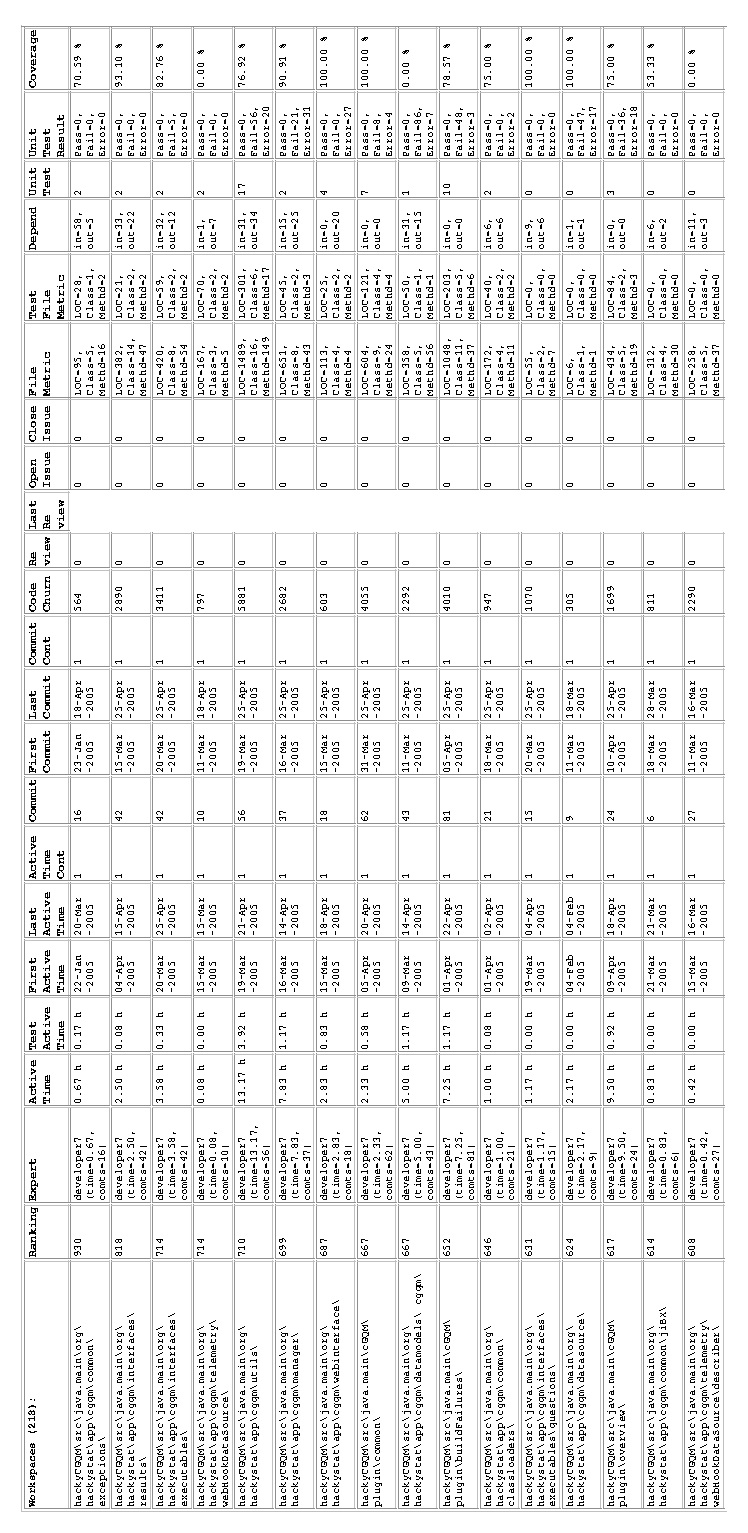
\includegraphics[totalheight=1.0\textheight]{figs/Results/11_2005-04-25-hackyCGQM-printable.eps}
  \label{fig:inspection11-hackyCGQM-ranking}
\end{figure}

\begin{figure}[!h]
  \centering
  \caption{hackyCGQM PRI Ranking - Inspection 11}
  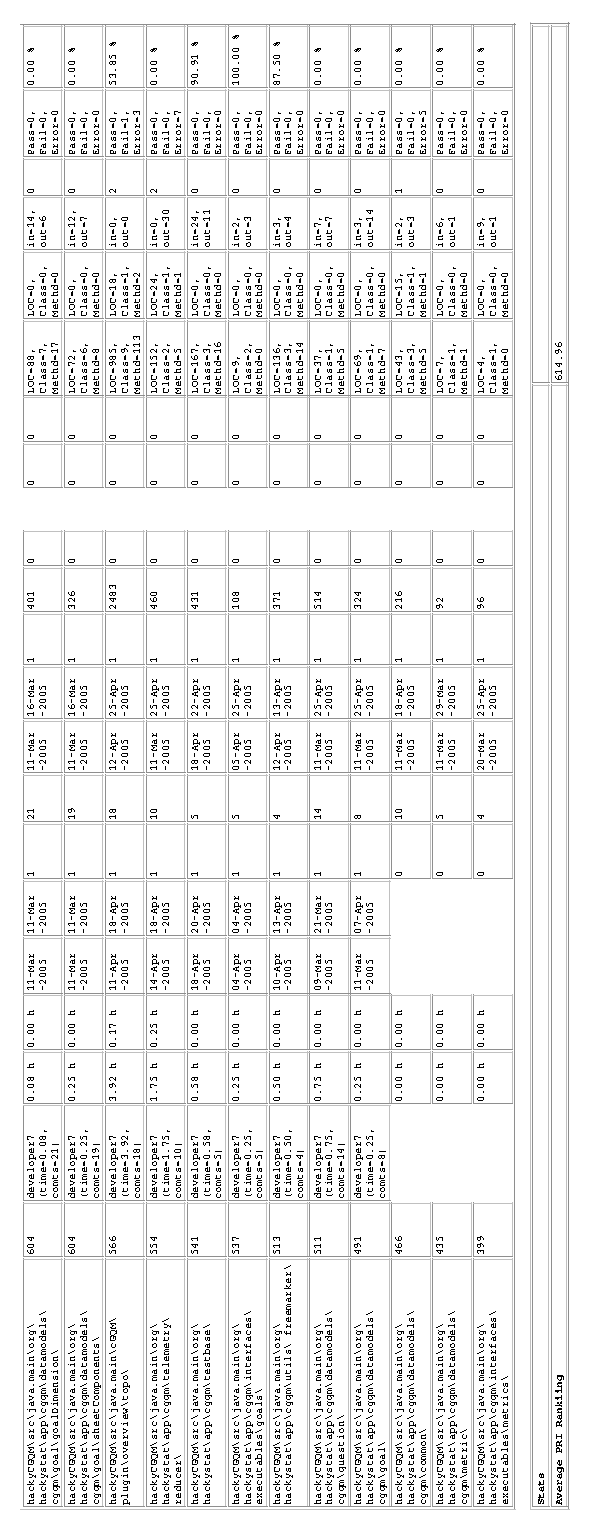
\includegraphics[totalheight=1.0\textheight]{figs/Results/11_2005-04-25-hackyCGQM-printable2.eps}
  \label{fig:inspection11-hackyCGQM-ranking-2}
\end{figure}


\clearpage
\subsection{hackyZorro}
The response to this question contains two results. First, a developer
ranking, which is provided in Table
\ref{tab:hackyZorro-developer-ranking}. Second, a PRI ranking, which is
provided in the Figure \ref{fig:inspection12-hackyZorro-ranking}.
Furthermore, the results of the developer rankings were used to help aid
the developer in selecting packages for inspection. Therefore, for
Inspection 12, the packages org.hackystat.stdext.zorro.control,
org.hackystat.stdext.zorror.control.stream, and
org.hackystat.stdext.zorro.model.action were selected. It appears that the
developer selected the control.stream and model.action packages to provide
examples of the use of control package. 

In this particular case, the developer ranking and PRI ranking disagreed
that the package was a MINI package, relative to other packages in the same
module. However, because only one inspection was conducted in this module,
it is not known whether the developer rankings or PRI rankings were
incorrect.

\begin{table}[!h]
  \begin{center}
    \caption{hackyZorro Developer Ranking}
    \label{tab:hackyZorro-developer-ranking}
    \begin{tabular}{|p{1.5cm}|p{11.5cm}|} \hline
{\bf Ranking} & {\bf Package} \\ \hline
1 & org.hackystat.stdext.zorro.analysis \\ \hline
2 & org.hackystat.stdext.zorro.control \\ \hline
3 & org.hackystat.stdext.zorro.control.tokenizer \\ \hline
4 & org.hackystat.stdext.zorro.jess \\ \hline
5 & org.hackystat.stdext.zorro.action.file.refactoring \\ \hline
6 & org.hackystat.stdext.zorro.model.episode \\ \hline
7 & org.hackystat.stdext.zorro.model.action.command \\ \hline
8 & org.hackystat.stdext.zorro.model.action.file.edit \\ \hline
9 & org.hackystat.stdext.zorro.control.stream \\ \hline
10 & org.hackystat.stdext.zorro.model.action.file \\ \hline
11 & org.hackystat.stdext.zorro.model.action \\ \hline
12 & org.hackystat.stdext.zorro.common \\ \hline
13 & org.hackystat.stdext.zorro.control.tokenizer.selector \\ \hline
14 & org.hackystat.stdext.zorro \\ \hline
    \end{tabular}
  \end{center}
\end{table}

\begin{figure}[!h]
  \centering
  \caption{hackyZorro PRI Ranking - Inspection 12}
  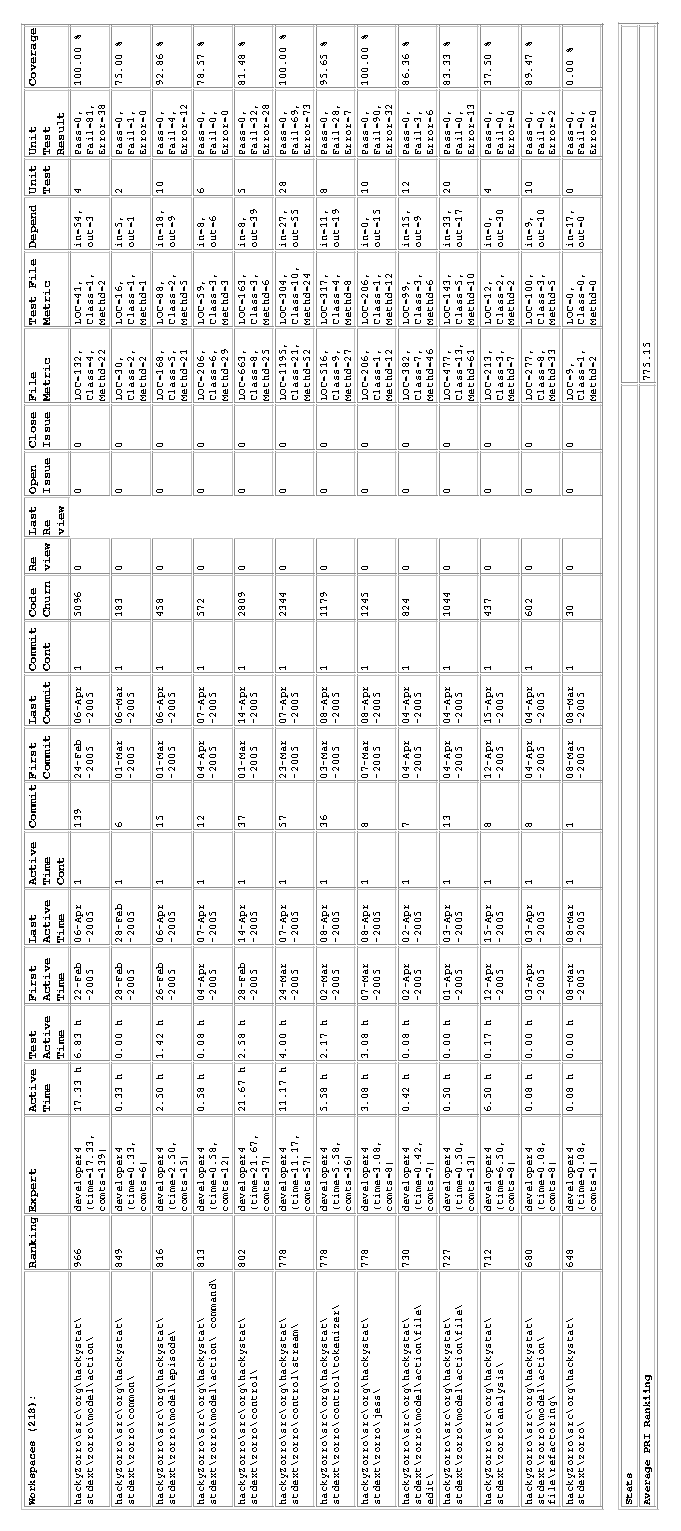
\includegraphics[totalheight=1.0\textheight]{figs/Results/12_2005-05-02-hackyZorro-printable.eps}
  \label{fig:inspection12-hackyZorro-ranking}
\end{figure}


\clearpage
\subsection{hackyTelemetry}
The response to this question contains two results. First, a developer
ranking, which is provided in Table
\ref{tab:hackyTelemetry-developer-ranking}. Second, a PRI ranking, which is
provided in the Figure \ref{fig:inspection14-hackyTelemetry-ranking}.
Furthermore, the results of the developer rankings were used to help aid
the developer in selecting a package for inspection. Therefore, for
Inspection 14, the package org.hackystat.app.telemetry.config was selected.

In this particular case, the developer ranking and PRI ranking disagreed
that the package was a MINI package, relative to other packages in the same
module. However, because only one inspection was conducted in this module,
it is not known whether the developer rankings or PRI rankings were
incorrect.

\begin{table}[!h]
  \begin{center}
    \caption{hackyTelemetry Developer Ranking}
    \label{tab:hackyTelemetry-developer-ranking}
    \begin{tabular}{|p{1.5cm}|p{11.5cm}|} \hline
{\bf Ranking} & {\bf Package} \\ \hline
1 & org.hackystat.app.telemetry.config \\ \hline
2 & org.hackystat.app.telemetry.analysis \\ \hline
3 & org.hackystat.app.telemetry.config.core \\ \hline
4 & org.hackystat.app.telemetry.processor.reducer.impl \\ \hline
5 & org.hackystat.app.telemetry.processor.parser.impl \\ \hline
6 & org.hackystat.app.telemetry.processor.evaluator \\ \hline
7 & org.hackystat.app.telemetry.processor.reducer.impl \\ \hline
8 & org.hackystat.app.telemetry.processor.query \\ \hline
9 & org.hackystat.app.telemetry.processor.parser \\ \hline
10 & org.hackystat.app.telemetry.processor.query.expression \\ \hline
11 & org.hackystat.app.telemetry.processor.reducer \\ \hline
12 & org.hackystat.app.telemetry.processor.stream \\ \hline
    \end{tabular}
  \end{center}
\end{table}


\begin{figure}[!h]
  \centering
  \caption{hackyTelemetry PRI Ranking - Inspection 14}
  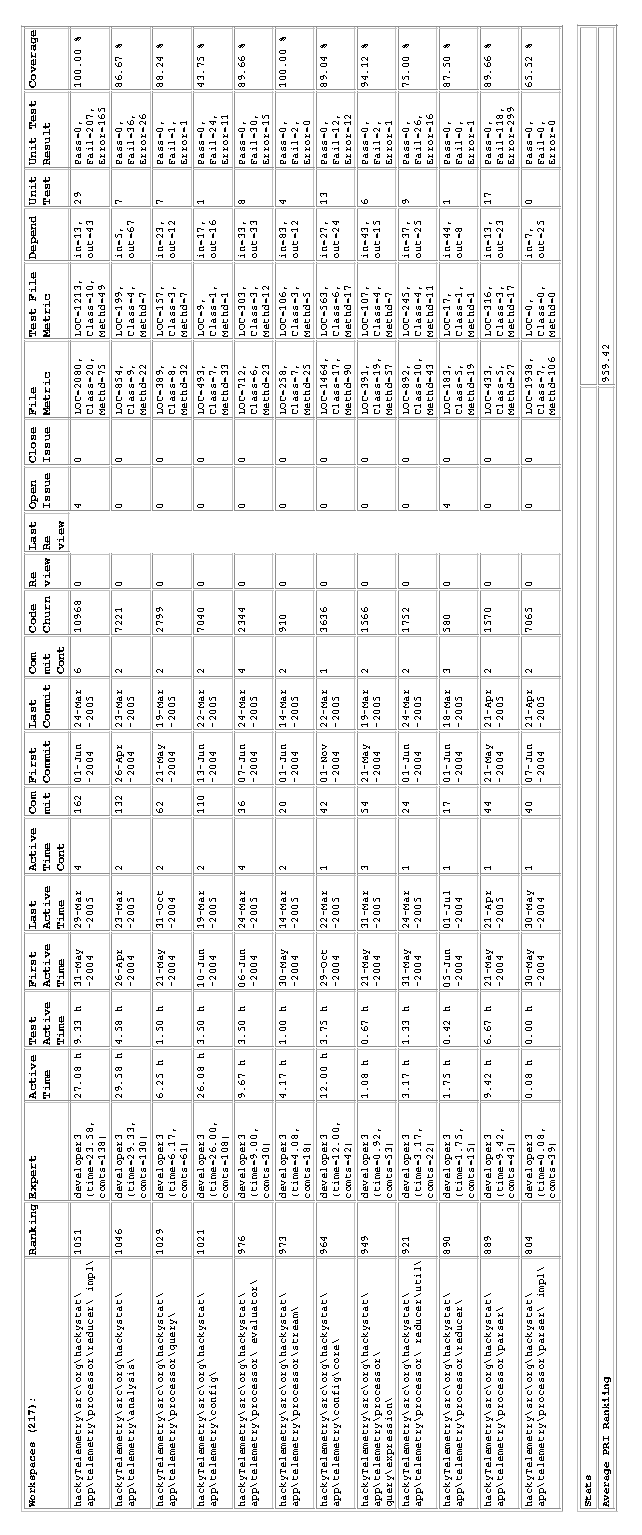
\includegraphics[totalheight=1.0\textheight]{figs/Results/14_2005-05-08-hackyTelemetry-printable.eps}
  \label{fig:inspection14-hackyTelemetry-ranking}
\end{figure}





\clearpage
\section{Question 8}
\label{appendix:section:question8}
\noindent \textbf{Question 8.} To the best of your knowledge, please
provide the top 5 modules that you think need to be inspected and the top 5 
modules that you think do NOT need to be inspected.

The Tables \ref{tab:pre-selection-questionnaire-results-8-p1},
\ref{tab:pre-selection-questionnaire-results-8-p2},
\ref{tab:pre-selection-questionnaire-results-8-p3},
\ref{tab:pre-selection-questionnaire-results-8-p4},
\ref{tab:pre-selection-questionnaire-results-8-p5}, and
\ref{tab:pre-selection-questionnaire-results-8-p6} present the results of
this question. Each table is one participants response. When available, I
provide the participants justification for giving a module a specific
ranking. ``??''  means that the participant could not provide an module.
``N/A'' means that the participant does not believe there is an appropriate
module.

Figures \ref{fig:pre-selection-questionnaire-results-8},
\ref{fig:pre-selection-questionnaire-results-82},
\ref{fig:pre-selection-questionnaire-results-8-explain}, and
\ref{fig:pre-selection-questionnaire-results-82-explain} provide a
graphical view of the responses.


\begin{table}[!h]
  \begin{center}
    \caption{Question 8 Responses - Participant 1}
    \label{tab:pre-selection-questionnaire-results-8-p1}
    \begin{tabular}{|p{2.0cm}|p{4.0cm}|p{7.0cm}|} \hline
{\bf Ranking} & {\bf Module} & {\bf Explanation} \\ \hline
\multicolumn{3}{|p{13.0cm}|}{Modules that need to be inspected} \\ \hline
1 & hackyCGQM & New code \\ \hline
2 & hackyZorro & New code \\ \hline
3 & hackyIssue & New code \\ \hline
4 & hackyDependency & New code \\ \hline
5 & ?? & \\ \hline
\multicolumn{3}{|p{13.0cm}|}{Modules that do not need to be inspected} \\ \hline
1 & hackyKernel & Old code \\ \hline
2 & hackyStdExt & Old code \\ \hline
3 & hackyStatistics & Old code \\ \hline
4 & hackyReport & Old code \\ \hline
5 & ?? & \\ \hline
    \end{tabular}
  \end{center}
\end{table}

\begin{table}[!h]
  \begin{center}
    \caption{Question 8 Responses - Participant 2}
    \label{tab:pre-selection-questionnaire-results-8-p2}
    \begin{tabular}{|p{2.0cm}|p{4.0cm}|p{7.0cm}|} \hline
{\bf Ranking} & {\bf Module} & {\bf Explanation} \\ \hline
\multicolumn{3}{|p{13.0cm}|}{Modules that need to be inspected} \\ \hline
1 & hackyCGQM & Causes many build failures \\ \hline
2 & hackyIssue & Knows there are defects in this code \\ \hline
3 & hackyZorro & New code \\ \hline
4 & ?? & \\ \hline
5 & ?? & \\ \hline
\multicolumn{3}{|p{13.0cm}|}{Modules that do not need to be inspected}  \\ \hline
1 & hackyJupiter & Fairly old code. No new development. Worked last year.\\ 
\hline
2 & hackyKernel & Core module. Used a lot. If there are problems, then it
would show up somewhere fast. \\ \hline
3 & hackyStdExt & Same as previous explanation \\ \hline
4 & ?? & \\ \hline
5 & ?? & \\ \hline
    \end{tabular}
  \end{center}
\end{table}


\begin{table}[!h]
  \begin{center}
    \caption{Question 8 Responses - Participant 3}
    \label{tab:pre-selection-questionnaire-results-8-p3}
    \begin{tabular}{|p{2.0cm}|p{4.0cm}|p{7.0cm}|} \hline
{\bf Ranking} & {\bf Module} & {\bf Explanation} \\ \hline
\multicolumn{3}{|p{13.0cm}|}{Modules that need to be inspected} \\ \hline
1 & hackyCGQM & Frequently fails build. New code. \\ \hline
2 & hackyZorro & Code has not been reviewed. \\ \hline
3 & hackyHPCS & Code has not been reviewed. \\ \hline
4 & hackyKernel & Important code \\ \hline
4 & hackyOffice & None of the office sensors work properly \\ \hline
\multicolumn{3}{|p{13.0cm}|}{Modules that do not need to be inspected}  \\ \hline
1 & N/A & No code should be excluded from inspection \\ \hline
2 & N/A & \\ \hline
3 & N/A & \\ \hline
4 & N/A & \\ \hline
5 & N/A & \\ \hline
    \end{tabular}
  \end{center}
\end{table}


\begin{table}[!h]
  \begin{center}
    \caption{Question 8 Responses - Participant 4}
    \label{tab:pre-selection-questionnaire-results-8-p4}
    \begin{tabular}{|p{2.0cm}|p{4.0cm}|p{7.0cm}|} \hline
{\bf Ranking} & {\bf Module} & {\bf Explanation} \\ \hline
\multicolumn{3}{|p{13.0cm}|}{Modules that need to be inspected} \\ \hline
1 & hackyEclipse & I don't trust the code. \\ \hline
2 & hackyCGQM & New code \\ \hline
3 & hackyZorro & New code \\ \hline
4 & hackyIssue & New code \\ \hline
5 & hackyPRI & New code \\ \hline
\multicolumn{3}{|p{13.0cm}|}{Modules that do not need to be inspected} \\ \hline
1 & hackyStatistics & Works fine. \\ \hline
2 & hackyVIM & No one uses it. Who cares? \\ \hline
3 & hackyTDD & No one uses it (after the new hackyZorro replaced it). Who
cares? \\ \hline 
4 & hackyCLI & No one uses it. Who Cares? \\ \hline
5 & hackyJBuilder & No one uses it. Who Cares? \\ \hline
    \end{tabular}
  \end{center}
\end{table}


\begin{table}[!h]
  \begin{center}
    \caption{Question 8 Responses - Participant 5}
    \label{tab:pre-selection-questionnaire-results-8-p5}
    \begin{tabular}{|p{2.0cm}|p{4.0cm}|p{7.0cm}|} \hline
{\bf Ranking} & {\bf Module} & {\bf Explanation} \\ \hline
\multicolumn{3}{|p{13.0cm}|}{Modules that need to be inspected} \\ \hline
1 & hackyStdExt & Large module and has many dependencies. \\ \hline
2 & hackyCGQM & New code and new developer. \\ \hline
3 & hackyIssue & I want to learn about the code. \\ \hline
4 & hackyTelemetry & Important code. Used a lot. \\ \hline
5 & hackyCLI & Could be useful, but we haven't paid any attention to it. \\ \hline
\multicolumn{3}{|p{13.0cm}|}{Modules that do not need to be inspected} \\ \hline
1 & hackyKernel & Important code, but we can detect errors quickly. \\ \hline
2 & hackyStatistics & Small module and its not used a lot. \\ \hline
3 & hackyReport & Been stable for a while. No new development. \\ \hline
4 & hackyEclipse & Been refactored. Has high use, so defects will be
found quickly. \\ \hline
5 & hackyPrjSize & No one uses it. Who Cares? \\ \hline
    \end{tabular}
  \end{center}
\end{table}



\begin{table}[!h]
  \begin{center}
    \caption{Question 8 Responses - Participant 6}
    \label{tab:pre-selection-questionnaire-results-8-p6}
    \begin{tabular}{|p{2.0cm}|p{4.0cm}|p{7.0cm}|} \hline
{\bf Ranking} & {\bf Module} & {\bf Explanation} \\ \hline
\multicolumn{3}{|p{13.0cm}|}{Modules that need to be inspected} \\ \hline
1 & hackyCGQM & Always fails the build. \\ \hline
2 & hackyZorro & Always fails the build. \\ \hline
3 & hackyStdExt & Always fails the build. \\ \hline
4 & ?? & \\ \hline
5 & ?? & \\ \hline
\multicolumn{3}{|p{13.0cm}|}{Modules that do not need to be inspected} \\ \hline
1 & hackyStatistics & Never fails the build. \\ \hline
2 & hackyReport & Never fails the build. \\ \hline
3 & ?? & \\ \hline
4 & ?? & \\ \hline
5 & ?? & \\ \hline
    \end{tabular}
  \end{center}
\end{table}


\clearpage
\begin{figure}[!h]
  \centering
  \includegraphics[width=1.0\textwidth]{figs/Results/pre-selection-questionnaire-8.eps}
  \caption[Question 8 Part 1 Responses]{Question 8 Part 1 Responses -
    Provides the total number of responses that the participants felt were
    MINI modules. ?? indicates that the participant did not know which
    module were MINI.}
  \label{fig:pre-selection-questionnaire-results-8}
\end{figure}

\begin{figure}[!h]
  \centering
  \includegraphics[width=1.0\textwidth]{figs/Results/pre-selection-questionnaire-82.eps}
  \caption[Question 8 Part 2 Responses]{Question 8 Part 2 Responses -
    Provides the total number of responses that the participants felt were
    LINI modules. ?? indicates that the participants did not know which
    modules were LINI. N/A indicates that the participants felt no module
    should be declared LINI.}
  \label{fig:pre-selection-questionnaire-results-82}
\end{figure}

\clearpage
\begin{figure}[!h]
  \centering
  \includegraphics[width=1.0\textwidth]{figs/Results/pre-selection-questionnaire-8-explain.eps}
  \caption[Question 8 Part 1 Responses]{Question 8 Part 1 Responses -
    Provides the total number of similar explanations used when ranking the 
    top 5 MINI modules.}
  \label{fig:pre-selection-questionnaire-results-8-explain}
\end{figure}

\begin{figure}[!h]
  \centering
  \includegraphics[width=1.0\textwidth]{figs/Results/pre-selection-questionnaire-82-explain.eps}
  \caption[Question 8 Part 2 Responses]{Question 8 Part 2 Responses -
    Provides the total number of similar explanations used when ranking the 
    top 5 LINI modules.}
  \label{fig:pre-selection-questionnaire-results-82-explain}
\end{figure}



\clearpage
\section{Question 9}
\label{appendix:section:question9}
\noindent \textbf{Question 9.} To the best of your knowledge, please
provide the top 5 workspaces that you think need to be inspected and the
top 5 workspaces that you think do NOT need to be inspected.

The Tables \ref{tab:pre-selection-questionnaire-results-9-p1},
\ref{tab:pre-selection-questionnaire-results-9-p2},
\ref{tab:pre-selection-questionnaire-results-9-p3},
\ref{tab:pre-selection-questionnaire-results-9-p4},
\ref{tab:pre-selection-questionnaire-results-9-p5}, and
\ref{tab:pre-selection-questionnaire-results-9-p6} present the results of
this question. Each table is one participants response. When available, I
provide the participants justification for giving a workspace a specific
ranking. ``??''  means that the participant could not provide an workspace.
``N/A'' means that the participant does not believe there is an appropriate
workspace.


\begin{table}[!h]
  \begin{center}
    \caption{Question 9 Responses - Participant 1}
    \label{tab:pre-selection-questionnaire-results-9-p1}
    \begin{tabular}{|p{2.0cm}|p{7.0cm}|p{4.0cm}|} \hline
{\bf Ranking} & {\bf Module} & {\bf Explanation} \\ \hline
\multicolumn{3}{|p{13.0cm}|}{Workspaces that need to be inspected} \\ \hline
1 & hackyCGQM/src/java.main/cGQM/ plugin/common & High Coverage \\ \hline
2 & hackyCGQM/src/org/hackystat/ app/cgqm/interfaces/executables/goals &
High Coverage \\ \hline 
3 & hackyCGQM/src/org/hackystat/ app/cgqm/interfaces/executables/questions
& High Coverage\\ \hline 
4 & hackyCli/src/org/hackystat/ app/cli/dailyanalysis & High Coverage \\ \hline
5 & ?? & \\ \hline
\multicolumn{3}{|p{13.0cm}|}{Workspaces that do not need to be inspected} \\ \hline
1 & hackyVCS/src/org/hackystat/ app/commit/analysis/projectchurn & Low Coverage \\ \hline
2 & hackyVCS/src/org/hackystat/ app/commit/dailyanalysis & Low Coverage \\ \hline
3 & hackyStdExt/src/org/hackystat/ stdext/bufftran/dailyanalysis & Low Coverage \\ \hline
4 & ?? & \\ \hline
5 & ?? & \\ \hline
    \end{tabular}
  \end{center}
\end{table}


\begin{table}[!h]
  \begin{center}
    \caption{Question 9 Responses - Participant 2}
    \label{tab:pre-selection-questionnaire-results-9-p2}
    \begin{tabular}{|p{2.0cm}|p{7.0cm}|p{4.0cm}|} \hline
{\bf Ranking} & {\bf Module} & {\bf Explanation} \\ \hline
\multicolumn{3}{|p{13.0cm}|}{Workspaces that need to be inspected} \\ \hline
1 & hackyCGQM/src/java.main/org/hackystat/ app/cgqm/manager & Package name
seems important \\ \hline
2 &
hackyCGQM/src/java.main/org/hackystat/ app/cgqm/telemetry/webHookDataSource
& Package name seems important \\ \hline 
3 &
hackyCGQM/src/java.main/org/hackystat/
app/cgqm/telemetry/webHookDataSource/ describer & Package name seems
important \\ \hline  
4 & hackyIssue/src/org/hackystat/ stdext/issue/reducer & New code. Known
issues. \\ \hline
5 & hackyAnt/src/org/hackystat/ stdext/sensor/ant/jira & New code. Important 
code. \\ \hline
\multicolumn{3}{|p{13.0cm}|}{Workspaces that do not need to be inspected} \\ \hline
1 & hackyKernel/src/org/hackystat/kernel/shell & Important code. \\ \hline
2 & hackyKernel/src/org/hackystat/kernel/shell/ command/ & Works correctly.
\\ \hline
3 & hackyKernel/src/org/hackystat/kernel/soap & Works correctly.  \\ \hline
4 & hackyKernel/src/org/hackystat/kernel/util & Works correctly.  \\ \hline
5 & hackyKernel/src/org/hackystat/kernel/timer & Works correctly.  \\ \hline
    \end{tabular}
  \end{center}
\end{table}


\begin{table}[!h]
  \begin{center}
    \caption{Question 9 Responses - Participant 3}
    \label{tab:pre-selection-questionnaire-results-9-p3}
    \begin{tabular}{|p{2.0cm}|p{7.0cm}|p{4.0cm}|} \hline
{\bf Ranking} & {\bf Module} & {\bf Explanation} \\ \hline
\multicolumn{3}{|p{13.0cm}|}{Workspaces that need to be inspected} \\ \hline
1 & hackyCQGM (any workspace) & No idea which workspace, but we should
inspect something in this module. \\ \hline
2 & hackyZorro (any workspace) & No idea which workspace, but we should
inspect something in this module. \\ \hline
3 & hackyHPCS/src/org/hackystat/ app/hpcs/dailyproject & Developed
quickly. \\ \hline
4 & hackyKernel/src/org/hackystat/kenrel/sdt & Before new improvements are
implemented \\ \hline
5 & hackyOffice (activity package) & Known issues. \\ \hline
\multicolumn{3}{|p{13.0cm}|}{Workspaces that do not need to be inspected} \\ \hline
1 & N/A & No code should be excluded from inspection \\ \hline
2 & N/A & \\ \hline
3 & N/A & \\ \hline
4 & N/A & \\ \hline
5 & N/A & \\ \hline
    \end{tabular}
  \end{center}
\end{table}

\begin{table}[!h]
  \begin{center}
    \caption{Question 9 Responses - Participant 4}
    \label{tab:pre-selection-questionnaire-results-9-p4}
    \begin{tabular}{|p{2.0cm}|p{7.0cm}|p{4.0cm}|} \hline
{\bf Ranking} & {\bf Module} & {\bf Explanation} \\ \hline
\multicolumn{3}{|p{13.0cm}|}{Workspaces that need to be inspected} \\ \hline
1 & ?? & I have no idea. \\ \hline
2 & ?? & \\ \hline
3 & ?? & \\ \hline
4 & ?? & \\ \hline
5 & ?? & \\ \hline
\multicolumn{3}{|p{13.0cm}|}{Workspaces that do not need to be inspected} \\ \hline
1 & ?? & I have no idea. \\ \hline
2 & ?? & \\ \hline
3 & ?? & \\ \hline
4 & ?? & \\ \hline
5 & ?? & \\ \hline
    \end{tabular}
  \end{center}
\end{table}


\begin{table}[!h]
  \begin{center}
    \caption{Question 9 Responses - Participant 5}
    \label{tab:pre-selection-questionnaire-results-9-p5}
    \begin{tabular}{|p{2.0cm}|p{7.0cm}|p{4.0cm}|} \hline
{\bf Ranking} & {\bf Module} & {\bf Explanation} \\ \hline
\multicolumn{3}{|p{13.0cm}|}{Workspaces that need to be inspected} \\ \hline
1 & hackyAnt/src/org/hackystat/ stdext/sensor/ant/junit & Known issues. \\ \hline
2 & hackyCGQM (any workspace) & Code standards. \\ \hline
3 & hackyIssue/src/org/hackystat/ sdtext/issue/reducer & Known issues. \\ \hline
4 & hackyReview/src/org/hackystat/ app/review/analysis/cache & Improvements
from last inspection. \\ \hline
5 & hackyZorro/src/org/hackystat/sdtext/zorro/jess & Known issues. \\ \hline
\multicolumn{3}{|p{13.0cm}|}{Workspaces that do not need to be inspected} \\ \hline
1 & hackyKernel/src/org/hackystat/kernel/util & Used widely. \\ \hline
2 & hackyKernel/src/org/hackystat/kernel/user & Used widely. \\ \hline
3 & hackyStatistics (any workspace)  & Not being used. Simple code. \\ \hline
4 & hackyReport (any workspace) & Used widely. \\ \hline
5 & hackyEclipse (any workspace) & Used widely. \\ \hline
    \end{tabular}
  \end{center}
\end{table}


\begin{table}[!h]
  \begin{center}
    \caption{Question 9 Responses - Participant 6}
    \label{tab:pre-selection-questionnaire-results-9-p6}
    \begin{tabular}{|p{2.0cm}|p{7.0cm}|p{4.0cm}|} \hline
{\bf Ranking} & {\bf Module} & {\bf Explanation} \\ \hline
\multicolumn{3}{|p{13.0cm}|}{Workspaces that need to be inspected} \\ \hline
1 & hackyCGQM (any workspace) & Many build failures. No idea which
workspace, but we should inspect something in this module. \\ \hline
2 & hackyZorro (any workspace) & Many build failures. No idea which
workspace, but we should inspect something in this module. \\ \hline
3 & ?? & \\ \hline
4 & ?? & \\ \hline
5 & ?? & \\ \hline
\multicolumn{3}{|p{13.0cm}|}{Workspaces that do not need to be inspected} \\ \hline
1 & hackyStatistics (any workspace) & \\ \hline
2 & hackyStatistics (any workspace) & \\ \hline
3 & hackyStatistics (any workspace) & \\ \hline
4 & hackyStatistics (any workspace) & \\ \hline
5 & hackyStatistics (any workspace) & \\ \hline
    \end{tabular}
  \end{center}
\end{table}






\chapter{Inspection and Post-Inspection-Questionnaire Results}
\label{appendix:chapter:inspection-results}




\section{Inspection 8}
\label{appendix:section:inspection8}


\begin{table}[!h]
  \begin{center}
    \caption[Inspection 8 - Package Details]{Inspection 8 - Package Details 
      - Provides various information about the package that was
      inspected. See other Tables and Figures in this chapter for more
      detailed information about the package.}
    \label{tab:inspection-package-details-8}
    \begin{tabular}{|p{5.0cm}|p{8.0cm}|} \hline
{\bf Package} & org.hackystat.stdext.review.analysis.cache \\ \hline
{\bf Module} & hackyReview \\ \hline
{\bf Developer Ranking} & MINI (See Table \ref{tab:hackyReview-developer-ranking}) \\ \hline
{\bf PRI Ranking} & MINI (See Figure \ref{fig:inspection8-hackyReview-ranking}) \\ \hline
{\bf Product and Process Measures} & See Figure \ref{fig:inspection8-hackyReview-ranking} \\ \hline
{\bf Inspection Date} & April 6, 2005 \\ \hline
{\bf Jupiter Review ID} & ReviewAnalysisCache \\ \hline
{\bf Number of Inspectors} & 5 \\ \hline
{\bf Meeting Attendance} & 7 \\ \hline
    \end{tabular}
  \end{center}
\end{table}


\begin{table}[!h]
  \begin{center}
    \caption[Inspection 8 - Results by Severity]{Inspection 8
      - Provides the valid defects found by the participants grouped by
      Severity.}
    \label{tab:inspection-results-8}
    \begin{tabular}{|p{2.0cm}|p{1.5cm}|p{1.5cm}|p{1.5cm}|p{1.5cm}|p{1.5cm}|p{1.5cm}|} \hline
{\bf Participant} & {\bf Critical} & {\bf Major} 
& {\bf Normal} & {\bf Minor} & {\bf Trivial} & {\bf Total} \\ \hline
1 &   &   & 1 &   & 1 & 2 \\ \hline
2 &   & 2 & 2 &   &   & 4 \\ \hline
3 &   &   & 2 & 1 & 2 & 5 \\ \hline
4 & 1 & 3 & 4 &   &   & 8 \\ \hline
5 &   & 2 & 2 & 1 &   & 5 \\ \hline
{\bf Total} & {\bf 1} & {\bf 7} & {\bf 11} & {\bf 2} & {\bf 3} & {\bf 24} \\ \hline
    \end{tabular}
  \end{center}
\end{table}


\begin{table}[!h]
  \begin{center}
    \caption[Inspection 8 - Results by Type and Severity]{Inspection 8 -
      Provides the valid defects found by the participants grouped by Type
      and Severity.}
    \label{tab:inspection-results-8-type}
    \begin{tabular}{|p{2.0cm}|p{1.7cm}|p{1.5cm}|p{1.7cm}|p{1.4cm}|p{1.4cm}|p{1.5cm}|}  \hline   
\small{} & \small{}{\bf Coding Standards} & 
\small{}{\bf Program Logic} & \small{} {\bf Optimi- zation} & 
\small{}{\bf Usability} & \small{} {\bf Clarity} & 
\small{} {\bf Suggestion} \\ \hline

{\bf Critical} &   & 1 &   &   &   &   \\ \hline
{\bf Major}    & 2 & 3 & 1 &   & 1 &   \\ \hline
{\bf Normal}   & 5 & 2 &   & 2 & 2 &   \\ \hline
{\bf Minor}    & 1 &   &   &   & 1 &   \\ \hline
{\bf Trivial}  & 2 &   &   &   & 1 &   \\ \hline

{\bf Total} & {\bf 10} & {\bf 6} & {\bf 1} & {\bf 2} & {\bf 5} & {\bf 0} \\ \hline
    \end{tabular}
  \end{center}
\end{table}

\begin{table}[!h]
  \begin{center}
    \caption[Post Inspection 8 - Responses]{Inspection 8 - Provides the
      responses from the Post-Inspection-Questionnaire}
    \label{tab:post-inspection-questionnaire-results-8}
    \begin{tabular}{|p{8.0cm}|p{2.5cm}|p{2.5cm}|} \hline
{\bf Question} & {\bf Yes} & {\bf No} \\ \hline
Did this package needed to be inspected?  & 5 & 2 \\ \hline
Did you learned something from this inspection?  & 5 & 2 \\ \hline
Did the inspection of this package increase its level of quality (once all
the issues are resolved)? & 7 & 0 \\ \hline
    \end{tabular}
  \end{center}
\end{table}





\clearpage
\section{Inspection 9}
\label{appendix:section:inspection9}


\begin{table}[!h]
  \begin{center}
    \caption[Inspection 9 - Package Details]{Inspection 9 - Package Details 
      - Provides various information about the package that was
      inspected. See other Tables and Figures in this chapter for more
      detailed information about the package.}
    \label{tab:inspection-package-details-8}
    \begin{tabular}{|p{5.0cm}|p{8.0cm}|} \hline
{\bf Package} & org.hackystat.stdext.issue.reducer \\ \hline
{\bf Module} & hackyIssue \\ \hline
{\bf Developer Ranking} & MINI (See Table \ref{tab:hackyIssue-developer-ranking}) \\ \hline
{\bf PRI Ranking} & MINI (See Figure \ref{fig:inspection9-hackyIssue-ranking}) \\ \hline
{\bf Product and Process Measures} & See Figure \ref{fig:inspection9-hackyIssue-ranking} \\ \hline
{\bf Inspection Date} & April 13, 2005 \\ \hline
{\bf Jupiter Review ID} & IssueReducer \\ \hline
{\bf Number of Inspectors} & 6 \\ \hline
{\bf Meeting Attendance} & 7 \\ \hline
    \end{tabular}
  \end{center}
\end{table}

\begin{table}[!h]
  \begin{center}
    \caption[Inspection 9 - Results by Severity]{Inspection 9
      - Provides the valid defects found by the participants grouped by
      Severity.}
    \label{tab:inspection-results-9}
    \begin{tabular}{|p{2.0cm}|p{1.5cm}|p{1.5cm}|p{1.5cm}|p{1.5cm}|p{1.5cm}|p{1.5cm}|} \hline
{\bf Participant} & {\bf Critical} & {\bf Major} 
& {\bf Normal} & {\bf Minor} & {\bf Trivial} & {\bf Total} \\ \hline
1 &   & 7 &   &   &   & 7 \\ \hline
2 &   &   & 1 & 3 &   & 4 \\ \hline
3 &   &   &   &   & 2 & 2 \\ \hline
4 &   & 2 & 7 &   &   & 9 \\ \hline
5 &   & 5 &   &   &   & 5 \\ \hline
6 &   & 2 & 5 & 1 & 2 & 10 \\ \hline
{\bf Total} & {\bf 0} & {\bf 16} & {\bf 13} & {\bf 4} & {\bf 4} & {\bf 37} \\ \hline
    \end{tabular}
  \end{center}
\end{table}


\begin{table}[!h]
  \begin{center}
    \caption[Inspection 9 - Results by Type and Severity]{Inspection 9 -
      Provides the valid defects found by the participants grouped by Type
      and Severity.}
    \label{tab:inspection-results-9-type}
    \begin{tabular}{|p{2.0cm}|p{1.7cm}|p{1.5cm}|p{1.7cm}|p{1.4cm}|p{1.4cm}|p{1.5cm}|}  \hline   
\small{} & \small{}{\bf Coding Standards} & 
\small{}{\bf Program Logic} & \small{} {\bf Optimi- zation} & 
\small{}{\bf Usability} & \small{} {\bf Clarity} & 
\small{} {\bf Suggestion} \\ \hline

{\bf Critical} &   &   &   &   &   &   \\ \hline
{\bf Major}    & 2 & 7 & 3 &   & 1 & 2 \\ \hline
{\bf Normal}   & 1 & 5 &   & 4 & 2 & 1  \\ \hline
{\bf Minor}    & 2 & 1 &   &   &   & 1 \\ \hline
{\bf Trivial}  & 4 &   &   &   &   &   \\ \hline

{\bf Total} & {\bf 9} & {\bf 13} & {\bf 3} & {\bf 4} & {\bf 3} & {\bf 4} \\ \hline
    \end{tabular}
  \end{center}
\end{table}



\begin{table}[!h]
  \begin{center}
    \caption[Post Inspection 9 - Responses]{Inspection 9 - Provides the
      responses from the Post-Inspection-Questionnaire}
    \label{tab:post-inspection-questionnaire-results-9}
    \begin{tabular}{|p{8.0cm}|p{2.5cm}|p{2.5cm}|} \hline
{\bf Question} & {\bf Yes} & {\bf No} \\ \hline
Did this package needed to be inspected?  & 7 & 0 \\ \hline
Did you learned something from this inspection?  & 7 & 0 \\ \hline
Did the inspection of this package increase its level of quality (once all
the issues are resolved)? & 7 & 0 \\ \hline
    \end{tabular}
  \end{center}
\end{table}


\clearpage
\section{Inspection 11}
\label{appendix:section:inspection11}

\begin{table}[!h]
  \begin{center}
    \caption[Inspection 11 - Package Details]{Inspection 11 - Package Details 
      - Provides various information about the package that was
      inspected. See other Tables and Figures in this chapter for more
      detailed information about the package.}
    \label{tab:inspection-package-details-11}
    \begin{tabular}{|p{5.0cm}|p{8.0cm}|} \hline
{\bf Packages} & org.hackystat.app.cgqm.interfaces.executables, \newline
org.hackystat.app.cgqm.interfaces.results, \newline
org.hackystat.app.cgqm.implementations.executables \\ \hline
{\bf Module} & hackyCGQM \\ \hline
{\bf Developer Ranking} & MINI (See Table \ref{tab:hackyCGQM-developer-ranking}) \\ \hline
{\bf PRI Ranking} & LINI (See Figure \ref{fig:inspection11-hackyCGQM-ranking}) \\ \hline
{\bf Product and Process Measures} & See Figure \ref{fig:inspection11-hackyCGQM-ranking} \\ \hline
{\bf Inspection Date} & April 27, 2005 \\ \hline
{\bf Jupiter Review ID} & cGQMInterfaces \\ \hline
{\bf Number of Inspectors} & 6 \\ \hline
{\bf Meeting Attendance} & 7 \\ \hline
    \end{tabular}
  \end{center}
\end{table}

\begin{table}[!h]
  \begin{center}
    \caption[Inspection 11 - Results by Severity]{Inspection 11
      - Provides the valid defects found by the participants grouped by
      Severity.}
    \label{tab:inspection-results-11}
    \begin{tabular}{|p{2.0cm}|p{1.5cm}|p{1.5cm}|p{1.5cm}|p{1.5cm}|p{1.5cm}|p{1.5cm}|} \hline
{\bf Participant} & {\bf Critical} & {\bf Major} 
& {\bf Normal} & {\bf Minor} & {\bf Trivial} & {\bf Total} \\ \hline
1 & 1 & 1 & 2 & 1 &   & 5 \\ \hline
2 &   & 5 & 2 &   &   & 7 \\ \hline
3 &   &   &   & 10&   & 10 \\ \hline
4 &   &   & 6 &   &   & 6 \\ \hline
5 &   & 5 & 3 &   & 1 & 9 \\ \hline
6 &   & 2 &   & 3 &   & 5 \\ \hline
{\bf Total} & {\bf 1} & {\bf 13} & {\bf 14} & {\bf 14} & {\bf 1} & {\bf 44} \\ \hline
    \end{tabular}
  \end{center}
\end{table}


\begin{table}[!h]
  \begin{center}
    \caption[Inspection 11 - Results by Type and Severity]{Inspection 11 -
      Provides the valid defects found by the participants grouped by Type
      and Severity.}
    \label{tab:inspection-results-11-type}
    \begin{tabular}{|p{2.0cm}|p{1.7cm}|p{1.5cm}|p{1.7cm}|p{1.4cm}|p{1.4cm}|p{1.5cm}|}  \hline   
\small{} & \small{}{\bf Coding Standards} & 
\small{}{\bf Program Logic} & \small{} {\bf Optimi- zation} & 
\small{}{\bf Usability} & \small{} {\bf Clarity} & 
\small{} {\bf Suggestion} \\ \hline

{\bf Critical} &   &   &   & 1 &   &   \\ \hline
{\bf Major}    & 2 & 6 & 2 & 1 &   & 3  \\ \hline
{\bf Normal}   & 8 & 1 & 1 &   &   & 3  \\ \hline
{\bf Minor}    & 11&   &   &   &   & 1  \\ \hline
{\bf Trivial}  & 1 &   &   &   &   &   \\ \hline

{\bf Total} & {\bf 22} & {\bf 7} & {\bf 3} & {\bf 2} & {\bf 0} & {\bf 7} \\ \hline

    \end{tabular}
  \end{center}
\end{table}



\begin{table}[!h]
  \begin{center}
    \caption[Post Inspection 11 - Responses]{Inspection 11 - Provides the
      responses from the Post-Inspection-Questionnaire}
    \label{tab:post-inspection-questionnaire-results-11}
    \begin{tabular}{|p{8.0cm}|p{2.5cm}|p{2.5cm}|} \hline
{\bf Question} & {\bf Yes} & {\bf No} \\ \hline
Did this package needed to be inspected?  & 6 & 1 \\ \hline
Did you learned something from this inspection?  & 7 & 0 \\ \hline
Did the inspection of this package increase its level of quality (once all
the issues are resolved)? & 7 & 0 \\ \hline
    \end{tabular}
  \end{center}
\end{table}


\clearpage
\section{Inspection 12}
\label{appendix:section:inspection12}

\begin{table}[!h]
  \begin{center}
    \caption[Inspection 12 - Package Details]{Inspection 12 - Package Details 
      - Provides various information about the package that was
      inspected. See other Tables and Figures in this chapter for more
      detailed information about the package.}
    \label{tab:inspection-package-details-12}
    \begin{tabular}{|p{5.0cm}|p{8.0cm}|} \hline
{\bf Packages} & org.hackystat.stdext.zorro.control \newline
org.hackystat.stdext.zorro.control.stream, \newline
org.hackystat.stdext.zorro..model.action \\ \hline
{\bf Module} & hackyZorro \\ \hline
{\bf Developer Ranking} & MINI (See Table \ref{tab:hackyZorro-developer-ranking}) \\ \hline
{\bf PRI Ranking} & LINI (See Figure \ref{fig:inspection12-hackyZorro-ranking}) \\ \hline
{\bf Product and Process Measures} & See Figure \ref{fig:inspection12-hackyZorro-ranking} \\ \hline
{\bf Inspection Date} & May 04, 2005 \\ \hline
{\bf Jupiter Review ID} & DevelopmentStream \\ \hline
{\bf Number of Inspectors} & 5 \\ \hline
{\bf Meeting Attendance} & 6 \\ \hline
    \end{tabular}
  \end{center}
\end{table}


\begin{table}[!h]
  \begin{center}
    \caption[Inspection 12 - Results by Severity]{Inspection 12
      - Provides the valid defects found by the participants grouped by
      Severity.}
    \label{tab:inspection-results-12}
    \begin{tabular}{|p{2.0cm}|p{1.5cm}|p{1.5cm}|p{1.5cm}|p{1.5cm}|p{1.5cm}|p{1.5cm}|} \hline
{\bf Participant} & {\bf Critical} & {\bf Major} 
& {\bf Normal} & {\bf Minor} & {\bf Trivial} & {\bf Total} \\ \hline
1 &   & 3 & 4 & 1 &   & 8 \\ \hline
2 &   & 2 & 3 & 1 &   & 6 \\ \hline
3 &   & 3 & 3 & 1 &   & 7 \\ \hline
4 &   & 2 & 2 & 3 &   & 7 \\ \hline
5 &   & 3 &   &   &   & 3 \\ \hline
{\bf Total} & {\bf 0} & {\bf 13} & {\bf 12} & {\bf 6} & {\bf 0} & {\bf 31} \\ \hline
    \end{tabular}
  \end{center}
\end{table}

\begin{table}[!h]
  \begin{center}
    \caption[Inspection 12 - Results by Type and Severity]{Inspection 12 -
      Provides the valid defects found by the participants grouped by Type
      and Severity.}
    \label{tab:inspection-results-12-type}
    \begin{tabular}{|p{2.0cm}|p{1.7cm}|p{1.5cm}|p{1.7cm}|p{1.4cm}|p{1.4cm}|p{1.5cm}|}  \hline   
\small{} & \small{}{\bf Coding Standards} & 
\small{}{\bf Program Logic} & \small{} {\bf Optimi- zation} & 
\small{}{\bf Usability} & \small{} {\bf Clarity} & 
\small{} {\bf Suggestion} \\ \hline

{\bf Critical} &   &   &   &   &   &   \\ \hline
{\bf Major}    & 1 & 4 & 1 & 2 & 3 & 2 \\ \hline
{\bf Normal}   & 7 &   &   & 2 & 3 &   \\ \hline
{\bf Minor}    & 6 &   &   &   &   &   \\ \hline
{\bf Trivial}  &   &   &   &   &   &   \\ \hline

{\bf Total} & {\bf 14} & {\bf 4} & {\bf 1} & {\bf 4} & {\bf 6} & {\bf 2} \\ \hline

    \end{tabular}
  \end{center}
\end{table}


\begin{table}[!h]
  \begin{center}
    \caption[Post Inspection 12 - Responses]{Inspection 12 - Provides the
      responses from the Post-Inspection-Questionnaire}
    \label{tab:post-inspection-questionnaire-results-12}
    \begin{tabular}{|p{8.0cm}|p{2.5cm}|p{2.5cm}|} \hline
{\bf Question} & {\bf Yes} & {\bf No} \\ \hline
Did this package needed to be inspected?  & 5 & 1 \\ \hline
Did you learned something from this inspection?  & 3 & 3 \\ \hline
Did the inspection of this package increase its level of quality (once all
the issues are resolved)? & 5 & 1 \\ \hline
    \end{tabular}
  \end{center}
\end{table}


\clearpage
\section{Inspection 13}
\label{appendix:section:inspection13}

\begin{table}[!h]
  \begin{center}
    \caption[Inspection 13 - Package Details]{Inspection 13 - Package Details 
      - Provides various information about the package that was
      inspected. See other Tables and Figures in this chapter for more
      detailed information about the package.}
    \label{tab:inspection-package-details-13}
    \begin{tabular}{|p{5.0cm}|p{8.0cm}|} \hline
{\bf Packages} & org.hackystat.stdext.issue.reducer \\ \hline
{\bf Module} & hackyIssue \\ \hline
{\bf Developer Ranking} & Second review of this package \\ \hline
{\bf PRI Ranking} & LINI (See Figure \ref{fig:inspection13-hackyIssue-ranking}) \\ \hline
{\bf Product and Process Measures} & See Figure \ref{fig:inspection13-hackyIssue-ranking} \\ \hline
{\bf Inspection Date} & May 4, 2005 \\ \hline
{\bf Jupiter Review ID} & IssueReducer2 \\ \hline
{\bf Number of Inspectors} & 4 \\ \hline
{\bf Meeting Attendance} & 6 \\ \hline
    \end{tabular}
  \end{center}
\end{table}


\begin{table}[!h]
  \begin{center}
    \caption[Inspection 13 - Results by Severity]{Inspection 13
      - Provides the valid defects found by the participants grouped by
      Severity.}
    \label{tab:inspection-results-13}
    \begin{tabular}{|p{2.0cm}|p{1.5cm}|p{1.5cm}|p{1.5cm}|p{1.5cm}|p{1.5cm}|p{1.5cm}|} \hline
{\bf Participant} & {\bf Critical} & {\bf Major} 
& {\bf Normal} & {\bf Minor} & {\bf Trivial} & {\bf Total} \\ \hline
1 &   & 1 &   &   &   & 1 \\ \hline
2 &   & 5 & 1 &   &   & 6 \\ \hline
3 & 1 &   &   &   &   & 0 \\ \hline
4 &   & 1 &   & 2 &   & 3 \\ \hline
{\bf Total} & {\bf 1} & {\bf 7} & {\bf 1} & {\bf 2} & {\bf 0} & {\bf 11} \\ \hline
    \end{tabular}
  \end{center}
\end{table}

\begin{table}[!h]
  \begin{center}
    \caption[Inspection 13 - Results by Type and Severity]{Inspection 13 -
      Provides the valid defects found by the participants grouped by Type
      and Severity.}
    \label{tab:inspection-results-13-type}
    \begin{tabular}{|p{2.0cm}|p{1.7cm}|p{1.5cm}|p{1.7cm}|p{1.4cm}|p{1.4cm}|p{1.5cm}|}  \hline   
\small{} & \small{}{\bf Coding Standards} & 
\small{}{\bf Program Logic} & \small{} {\bf Optimi- zation} & 
\small{}{\bf Usability} & \small{} {\bf Clarity} & 
\small{} {\bf Suggestion} \\ \hline

{\bf Critical} &   & 1 &   &   &   &   \\ \hline
{\bf Major}    & 3 & 4 &   &   &   &   \\ \hline
{\bf Normal}   &   & 1 &   &   &   &   \\ \hline
{\bf Minor}    & 2 &   &   &   &   &   \\ \hline
{\bf Trivial}  &   &   &   &   &   &   \\ \hline

{\bf Total} & {\bf 5} & {\bf 6} & {\bf 0} & {\bf 0} & {\bf 0} & {\bf 0} \\ \hline
    \end{tabular}
  \end{center}
\end{table}


\begin{table}[!h]
  \begin{center}
    \caption[Post Inspection 13 - Responses]{Inspection 13 - Provides the
      responses from the Post-Inspection-Questionnaire}
    \label{tab:post-inspection-questionnaire-results-13}
    \begin{tabular}{|p{8.0cm}|p{2.5cm}|p{2.5cm}|} \hline
{\bf Question} & {\bf Yes} & {\bf No} \\ \hline
Did this package needed to be inspected?  & 3 & 3 \\ \hline
Did you learned something from this inspection?  & 3 & 3 \\ \hline
Did the inspection of this package increase its level of quality (once all
the issues are resolved)? & 4 & 2 \\ \hline
    \end{tabular}
  \end{center}
\end{table}

\begin{figure}[htb]
  \centering
  \caption{hackyIssue PRI Ranking - Inspection 13}
  \includegraphics[totalheight=1.0\textheight]{figs/Results/13_2005-05-02-hackyIssue-printable.eps}
  \label{fig:inspection13-hackyIssue-ranking}
\end{figure}


\clearpage
\section{Inspection 14}
\label{appendix:section:inspection14}

\begin{table}[!h]
  \begin{center}
    \caption[Inspection 14 - Package Details]{Inspection 14 - Package Details 
      - Provides various information about the package that was
      inspected. See other Tables and Figures in this chapter for more
      detailed information about the package.}
    \label{tab:inspection-package-details-14}
    \begin{tabular}{|p{5.0cm}|p{8.0cm}|} \hline
{\bf Packages} & org.hackystat.app.telemetry.config \\ \hline
{\bf Module} & hackyTelemetry \\ \hline
{\bf Developer Ranking} & MINI (See Table \ref{tab:hackyTelemetry-developer-ranking}) \\ \hline
{\bf PRI Ranking} & LINI (See Figure \ref{fig:inspection14-hackyTelemetry-ranking}) \\ \hline
{\bf Product and Process Measures} & See Figure \ref{fig:inspection14-hackyTelemetry-ranking} \\ \hline
{\bf Inspection Date} & May 11, 2005 \\ \hline
{\bf Jupiter Review ID} & TelemetryWebConfig \\ \hline
{\bf Number of Inspectors} & 6 \\ \hline
{\bf Meeting Attendance} & 6 \\ \hline
    \end{tabular}
  \end{center}
\end{table}

\begin{table}[!h]
  \begin{center}
    \caption[Inspection 14 - Results by Severity]{Inspection 14
      - Provides the valid defects found by the participants grouped by
      Severity.}
    \label{tab:inspection-results-14}
    \begin{tabular}{|p{2.0cm}|p{1.5cm}|p{1.5cm}|p{1.5cm}|p{1.5cm}|p{1.5cm}|p{1.5cm}|} \hline
{\bf Participant} & {\bf Critical} & {\bf Major} 
& {\bf Normal} & {\bf Minor} & {\bf Trivial} & {\bf Total} \\ \hline
1 &   & 1 & 4 &   &   & 5 \\ \hline
2 & 1 & 2 &   &   &   & 3 \\ \hline
3 &   & 1 & 2 &   &   & 3 \\ \hline
4 &   & 3 & 4 &   &   & 7 \\ \hline
5 &   & 4 & 1 &   &   & 5 \\ \hline
6 &   & 2 & 1 &   &   & 3 \\ \hline
{\bf Total} & {\bf 1} & {\bf 13} & {\bf 12} & {\bf 0} & {\bf 0} & {\bf 26} \\ \hline
    \end{tabular}
  \end{center}
\end{table}

\begin{table}[!h]
  \begin{center}
    \caption[Inspection 14 - Results by Type and Severity]{Inspection 14 -
      Provides the valid defects found by the participants grouped by Type
      and Severity.}
    \label{tab:inspection-results-14-type}
    \begin{tabular}{|p{2.0cm}|p{1.7cm}|p{1.5cm}|p{1.7cm}|p{1.4cm}|p{1.4cm}|p{1.5cm}|}  \hline   
\small{} & \small{}{\bf Coding Standards} & 
\small{}{\bf Program Logic} & \small{} {\bf Optimi- zation} & 
\small{}{\bf Usability} & \small{} {\bf Clarity} & 
\small{} {\bf Suggestion} \\ \hline

{\bf Critical} &   & 1 &   &   &   &   \\ \hline
{\bf Major}    & 3 & 1 & 1 & 5 &   & 2 \\ \hline
{\bf Normal}   & 6 & 2 &   & 3 & 1 &   \\ \hline
{\bf Minor}    &   &   &   &   &   &   \\ \hline
{\bf Trivial}  &   &   &   &   &   &   \\ \hline

{\bf Total} & {\bf 9} & {\bf 4} & {\bf 1} & {\bf 8} & {\bf 1} & {\bf 2} \\ \hline
    \end{tabular}
  \end{center}
\end{table}



\begin{table}[!h]
  \begin{center}
    \caption[Post Inspection 14 - Responses]{Inspection 14 - Provides the
      responses from the Post-Inspection-Questionnaire}
    \label{tab:post-inspection-questionnaire-results-14}
    \begin{tabular}{|p{8.0cm}|p{2.5cm}|p{2.5cm}|} \hline
{\bf Question} & {\bf Yes} & {\bf No} \\ \hline
Did this package needed to be inspected?  & 6 & 0 \\ \hline
Did you learned something from this inspection?  & 6 & 0 \\ \hline
Did the inspection of this package increase its level of quality (once all
the issues are resolved)? & 6 & 0 \\ \hline
    \end{tabular}
  \end{center}
\end{table}


\clearpage
\section{Inspection 15}
\label{appendix:section:inspection15}

\begin{table}[!h]
  \begin{center}
    \caption[Inspection 15 - Package Details]{Inspection 15 - Package Details 
      - Provides various information about the package that was
      inspected. See other Tables and Figures in this chapter for more
      detailed information about the package.}
    \label{tab:inspection-package-details-15}
    \begin{tabular}{|p{5.0cm}|p{8.0cm}|} \hline
{\bf Packages} & org.hackystat.kernel.cache \\ \hline
{\bf Module} & hackyKernel \\ \hline
{\bf Developer Ranking} & N/A - hand selected via PRI ranking \\ \hline
{\bf PRI Ranking} & LINI (See Figure \ref{fig:inspection15-hackyKernel-ranking}) \\ \hline
{\bf Product and Process Measures} & See Figure \ref{fig:inspection15-hackyKernel-ranking} \\ \hline
{\bf Inspection Date} & June 1, 2005 \\ \hline
{\bf Jupiter Review ID} & KernelCache \\ \hline
{\bf Number of Inspectors} & 6 \\ \hline
{\bf Meeting Attendance} & 5 \\ \hline
    \end{tabular}
  \end{center}
\end{table}

\begin{table}[!h]
  \begin{center}
    \caption[Inspection 15 - Results by Severity]{Inspection 15
      - Provides the valid defects found by the participants grouped by
      Severity.}
    \label{tab:inspection-results-15}
    \begin{tabular}{|p{2.0cm}|p{1.5cm}|p{1.5cm}|p{1.5cm}|p{1.5cm}|p{1.5cm}|p{1.5cm}|} \hline
{\bf Participant} & {\bf Critical} & {\bf Major} 
& {\bf Normal} & {\bf Minor} & {\bf Trivial} & {\bf Total} \\ \hline
1 &   &   &   &   &   & 0 \\ \hline
2 &   & 1 &   &   &   & 1 \\ \hline
3 &   &   & 2 &   &   & 2 \\ \hline
4 &   &   & 3 & 2 &   & 5 \\ \hline
5 &   &   &   &   &   & 0 \\ \hline
6 &   &   & 1 &   & 1 & 2 \\ \hline
{\bf Total} & {\bf 0} & {\bf 1} & {\bf 6} & {\bf 2} & {\bf 1} & {\bf 10} \\ \hline
    \end{tabular}
  \end{center}
\end{table}

\begin{table}[!h]
  \begin{center}
    \caption[Inspection 15 - Results by Type and Severity]{Inspection 15 -
      Provides the valid defects found by the participants grouped by Type
      and Severity.}
    \label{tab:inspection-results-15-type}
    \begin{tabular}{|p{2.0cm}|p{1.7cm}|p{1.5cm}|p{1.7cm}|p{1.4cm}|p{1.4cm}|p{1.5cm}|}  \hline   
\small{} & \small{}{\bf Coding Standards} & 
\small{}{\bf Program Logic} & \small{} {\bf Optimi- zation} & 
\small{}{\bf Usability} & \small{} {\bf Clarity} & 
\small{} {\bf Suggestion} \\ \hline

{\bf Critical} &   &   &   &   &   &   \\ \hline
{\bf Major}    &   & 1 &   &   &   &   \\ \hline
{\bf Normal}   & 3 & 1 &   &   & 1 &   \\ \hline
{\bf Minor}    & 2 &   &   &   &   &   \\ \hline
{\bf Trivial}  & 1 &   &   &   &   &   \\ \hline

{\bf Total} & {\bf 6} & {\bf 2} & {\bf 0} & {\bf 0} & {\bf 1} & {\bf 0} \\ \hline
    \end{tabular}
  \end{center}
\end{table}


\begin{table}[!h]
  \begin{center}
    \caption[Post Inspection 15 - Responses]{Inspection 15 - Provides the
      responses from the Post-Inspection-Questionnaire}
    \label{tab:post-inspection-questionnaire-results-15}
    \begin{tabular}{|p{8.0cm}|p{2.5cm}|p{2.5cm}|} \hline
{\bf Question} & {\bf Yes} & {\bf No} \\ \hline
Did this package needed to be inspected?  & 2 & 3 \\ \hline
Did you learned something from this inspection?  & 4 & 1 \\ \hline
Did the inspection of this package increase its level of quality (once all
the issues are resolved)? & 4 & 1 \\ \hline
    \end{tabular}
  \end{center}
\end{table}

\begin{figure}[htb]
  \centering
  \caption{hackyKernel PRI Ranking - Inspection 15}
  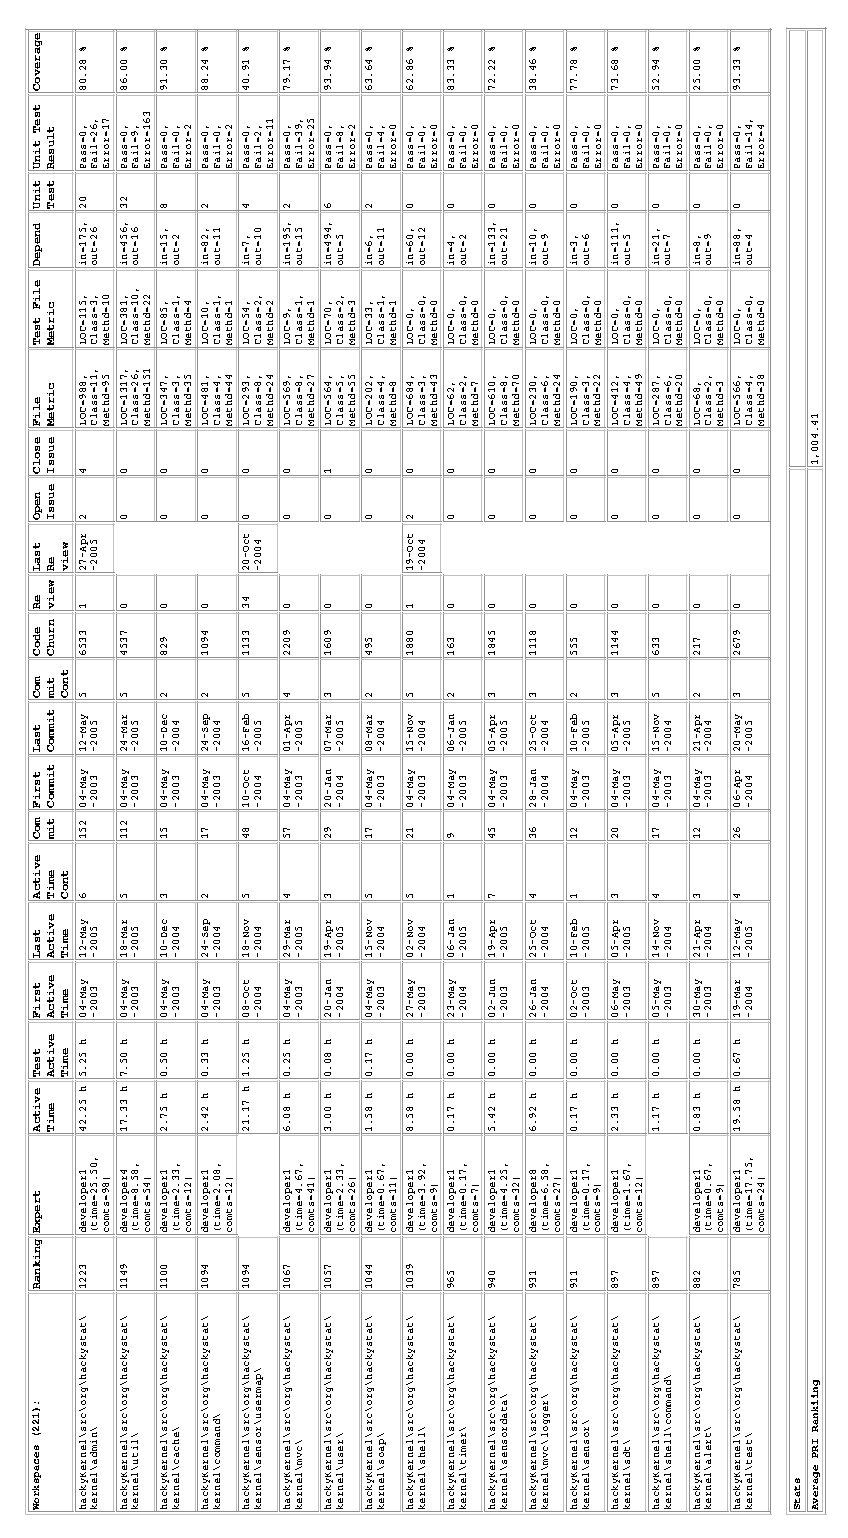
\includegraphics[totalheight=1.0\textheight]{figs/Results/15_2005-05-25-hackyKernel-printable.eps}
  \label{fig:inspection15-hackyKernel-ranking}
\end{figure}




\clearpage
\section{Inspection 16}
\label{appendix:section:inspection16}

\begin{table}[!h]
  \begin{center}
    \caption[Inspection 16 - Package Details]{Inspection 16 - Package Details 
      - Provides various information about the package that was
      inspected. See other Tables and Figures in this chapter for more
      detailed information about the package.}
    \label{tab:inspection-package-details-16}
    \begin{tabular}{|p{5.0cm}|p{8.0cm}|} \hline
{\bf Packages} & org.hackystat.stdext.project \\ \hline
{\bf Module} & hackyStdExt \\ \hline
{\bf Developer Ranking} & N/A - hand selected via PRI ranking \\ \hline
{\bf PRI Ranking} & LINI (See Figure \ref{fig:inspection16-hackyStdExt-ranking}) \\ \hline
{\bf Product and Process Measures} & See Figure \ref{fig:inspection16-hackyStdExt-ranking} \\ \hline
{\bf Inspection Date} & June 1, 2005 \\ \hline
{\bf Jupiter Review ID} & Project \\ \hline
{\bf Number of Inspectors} & 5 \\ \hline
{\bf Meeting Attendance} & 5 \\ \hline
    \end{tabular}
  \end{center}
\end{table}

\begin{table}[!h]
  \begin{center}
    \caption[Inspection 16 - Results by Severity]{Inspection 16
      - Provides the valid defects found by the participants grouped by
      Severity.}
    \label{tab:inspection-results-16}
    \begin{tabular}{|p{2.0cm}|p{1.5cm}|p{1.5cm}|p{1.5cm}|p{1.5cm}|p{1.5cm}|p{1.5cm}|} \hline
{\bf Participant} & {\bf Critical} & {\bf Major} 
& {\bf Normal} & {\bf Minor} & {\bf Trivial} & {\bf Total} \\ \hline
1 &   & 1 & 2 & 1 &   & 4 \\ \hline
2 &   &   &   &   &   & 0 \\ \hline
3 &   &   &   &   & 1 & 1 \\ \hline
4 &   & 1 &   &   & 1 & 2 \\ \hline
5 &   & 1 & 2 &   &   & 3 \\ \hline
{\bf Total} & {\bf 0} & {\bf 3} & {\bf 4} & {\bf 3} & {\bf 0} & {\bf 10} \\ \hline
    \end{tabular}
  \end{center}
\end{table}

\begin{table}[!h]
  \begin{center}
    \caption[Inspection 16 - Results by Type and Severity]{Inspection 16 -
      Provides the valid defects found by the participants grouped by Type
      and Severity.}
    \label{tab:inspection-results-16-type}
    \begin{tabular}{|p{2.0cm}|p{1.7cm}|p{1.5cm}|p{1.7cm}|p{1.4cm}|p{1.4cm}|p{1.5cm}|}  \hline   
\small{} & \small{}{\bf Coding Standards} & 
\small{}{\bf Program Logic} & \small{} {\bf Optimi- zation} & 
\small{}{\bf Usability} & \small{} {\bf Clarity} & 
\small{} {\bf Suggestion} \\ \hline

{\bf Critical} &   &   &   &   &   &   \\ \hline
{\bf Major}    &   &   & 1 &   & 1 & 1 \\ \hline
{\bf Normal}   &   &   &   & 1 & 2 &   \\ \hline
{\bf Minor}    &   &   & 1 &   &   & 2 \\ \hline
{\bf Trivial}  &   &   &   &   &   &   \\ \hline

{\bf Total} & {\bf 0} & {\bf 0} & {\bf 2} & {\bf 1} & {\bf 3} & {\bf 3} \\ \hline
    \end{tabular}
  \end{center}
\end{table}


\begin{table}[!h]
  \begin{center}
    \caption[Post Inspection 16 - Responses]{Inspection 16 - Provides the
      responses from the Post-Inspection-Questionnaire}
    \label{tab:post-inspection-questionnaire-results-16}
    \begin{tabular}{|p{8.0cm}|p{2.5cm}|p{2.5cm}|} \hline
{\bf Question} & {\bf Yes} & {\bf No} \\ \hline
Did this package needed to be inspected?  & 3 & 2 \\ \hline
Did you learned something from this inspection?  & 4 & 1 \\ \hline
Did the inspection of this package increase its level of quality (once all
the issues are resolved)? & 4 & 1 \\ \hline
    \end{tabular}
  \end{center}
\end{table}

\begin{figure}[htb]
  \centering
  \caption{hackyStdExt PRI Ranking - Inspection 16}
  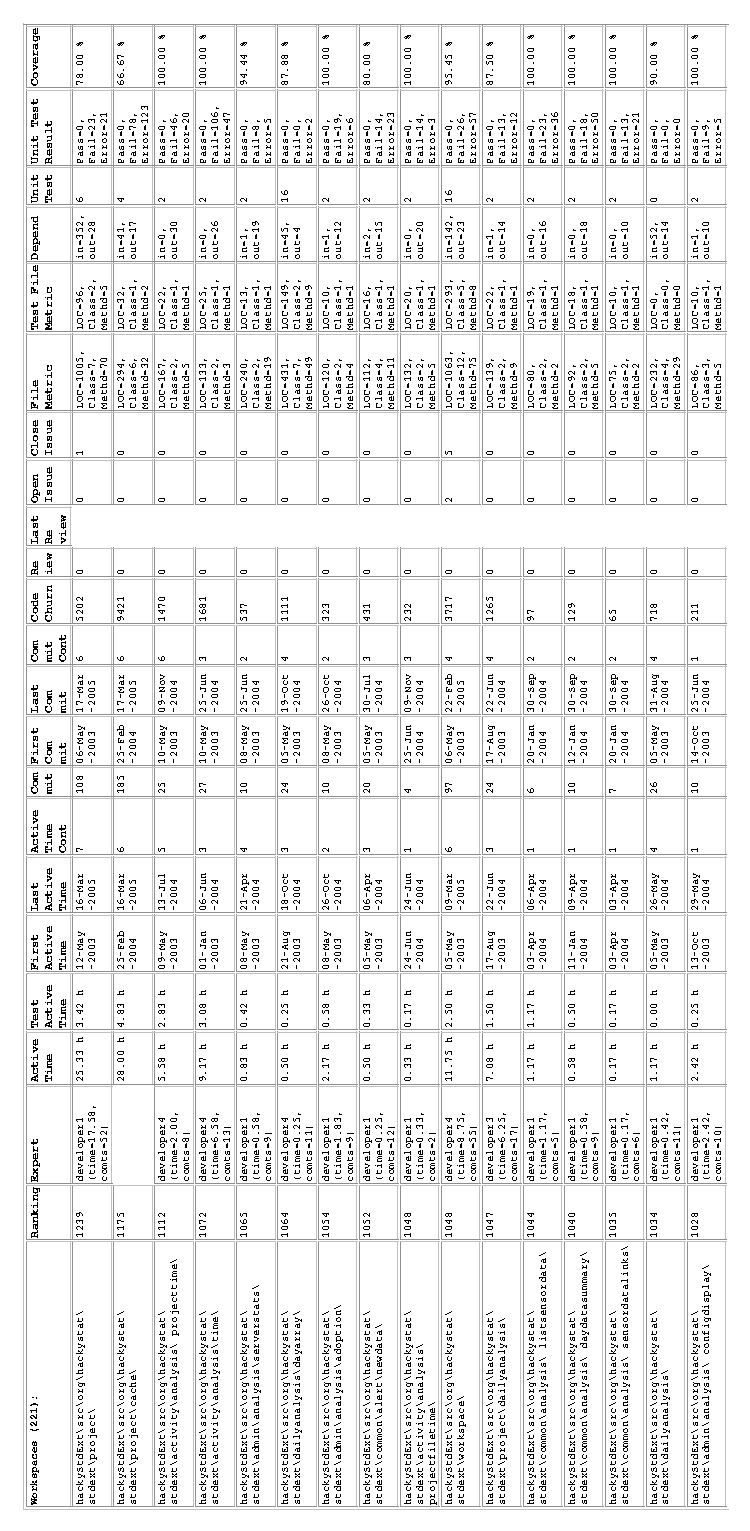
\includegraphics[totalheight=1.0\textheight]{figs/Results/16_2005-05-25-hackyStdExt-printable.eps}
  \label{fig:inspection16-hackyStdExt-ranking}
\end{figure}



\clearpage
\section{Inspection 17}
\label{appendix:section:inspection17}

\begin{table}[!h]
  \begin{center}
    \caption[Inspection 17 - Package Details]{Inspection 17 - Package Details 
      - Provides various information about the package that was
      inspected. See other Tables and Figures in this chapter for more
      detailed information about the package.}
    \label{tab:inspection-package-details-17}
    \begin{tabular}{|p{5.0cm}|p{8.0cm}|} \hline
{\bf Packages} & org.hackystat.stdext.project.cache \\ \hline
{\bf Module} & hackyStdExt \\ \hline
{\bf Developer Ranking} & N/A - hand selected via PRI ranking \\ \hline
{\bf PRI Ranking} & LINI (See Figure \ref{fig:inspection17-hackyStdExt-ranking}) \\ \hline
{\bf Product and Process Measures} & See Figure \ref{fig:inspection17-hackyStdExt-ranking} \\ \hline
{\bf Inspection Date} & June 8, 2005 \\ \hline
{\bf Jupiter Review ID} & ProjectCache \\ \hline
{\bf Number of Inspectors} & 5 \\ \hline
{\bf Meeting Attendance} & 4 \\ \hline
    \end{tabular}
  \end{center}
\end{table}

\begin{table}[!h]
  \begin{center}
    \caption[Inspection 17 - Results by Severity]{Inspection 17
      - Provides the valid defects found by the participants grouped by
      Severity.}
    \label{tab:inspection-results-17}
    \begin{tabular}{|p{2.0cm}|p{1.5cm}|p{1.5cm}|p{1.5cm}|p{1.5cm}|p{1.5cm}|p{1.5cm}|} \hline
{\bf Participant} & {\bf Critical} & {\bf Major} 
& {\bf Normal} & {\bf Minor} & {\bf Trivial} & {\bf Total} \\ \hline
1 &   & 1 & 3 &   &   & 4 \\ \hline
2 &   & 1 &   &   &   & 1 \\ \hline
3 &   & 3 & 1 & 1 & 2 & 7 \\ \hline
4 &   & 1 & 2 &   & 1 & 4 \\ \hline
5 &   & 1 &   &   &   & 1 \\ \hline
{\bf Total} & {\bf 0} & {\bf 7} & {\bf 6} & {\bf 1} & {\bf 3} & {\bf 17} \\ \hline
    \end{tabular}
  \end{center}
\end{table}

\begin{table}[!h]
  \begin{center}
    \caption[Inspection 17 - Results by Type and Severity]{Inspection 17 -
      Provides the valid defects found by the participants grouped by Type
      and Severity.}
    \label{tab:inspection-results-17-type}
    \begin{tabular}{|p{2.0cm}|p{1.7cm}|p{1.5cm}|p{1.7cm}|p{1.4cm}|p{1.4cm}|p{1.5cm}|}  \hline   
\small{} & \small{}{\bf Coding Standards} & 
\small{}{\bf Program Logic} & \small{} {\bf Optimi- zation} & 
\small{}{\bf Usability} & \small{} {\bf Clarity} & 
\small{} {\bf Suggestion} \\ \hline

{\bf Critical} &   &   &   &   &   &   \\ \hline
{\bf Major}    &   & 2 & 2 &   &   &   \\ \hline
{\bf Normal}   & 1 &   & 3 &   & 2 &   \\ \hline
{\bf Minor}    &   &   &   &   &   &   \\ \hline
{\bf Trivial}  & 1 &   &   &   &   &   \\ \hline

{\bf Total} & {\bf 2} & {\bf 2} & {\bf 5} & {\bf 0} & {\bf 2} & {\bf 0} \\ \hline
    \end{tabular}
  \end{center}
\end{table}


\begin{table}[!h]
  \begin{center}
    \caption[Post Inspection 17 - Responses]{Inspection 17 - Provides the
      responses from the Post-Inspection-Questionnaire}
    \label{tab:post-inspection-questionnaire-results-17}
    \begin{tabular}{|p{8.0cm}|p{2.5cm}|p{2.5cm}|} \hline
{\bf Question} & {\bf Yes} & {\bf No} \\ \hline
Did this package needed to be inspected?  & 2 & 2 \\ \hline
Did you learned something from this inspection?  & 3 & 1 \\ \hline
Did the inspection of this package increase its level of quality (once all
the issues are resolved)? & 4 & 0 \\ \hline
    \end{tabular}
  \end{center}
\end{table}


\begin{figure}[htb]
  \centering
  \caption{hackyStdExt PRI Ranking - Inspection 17}
  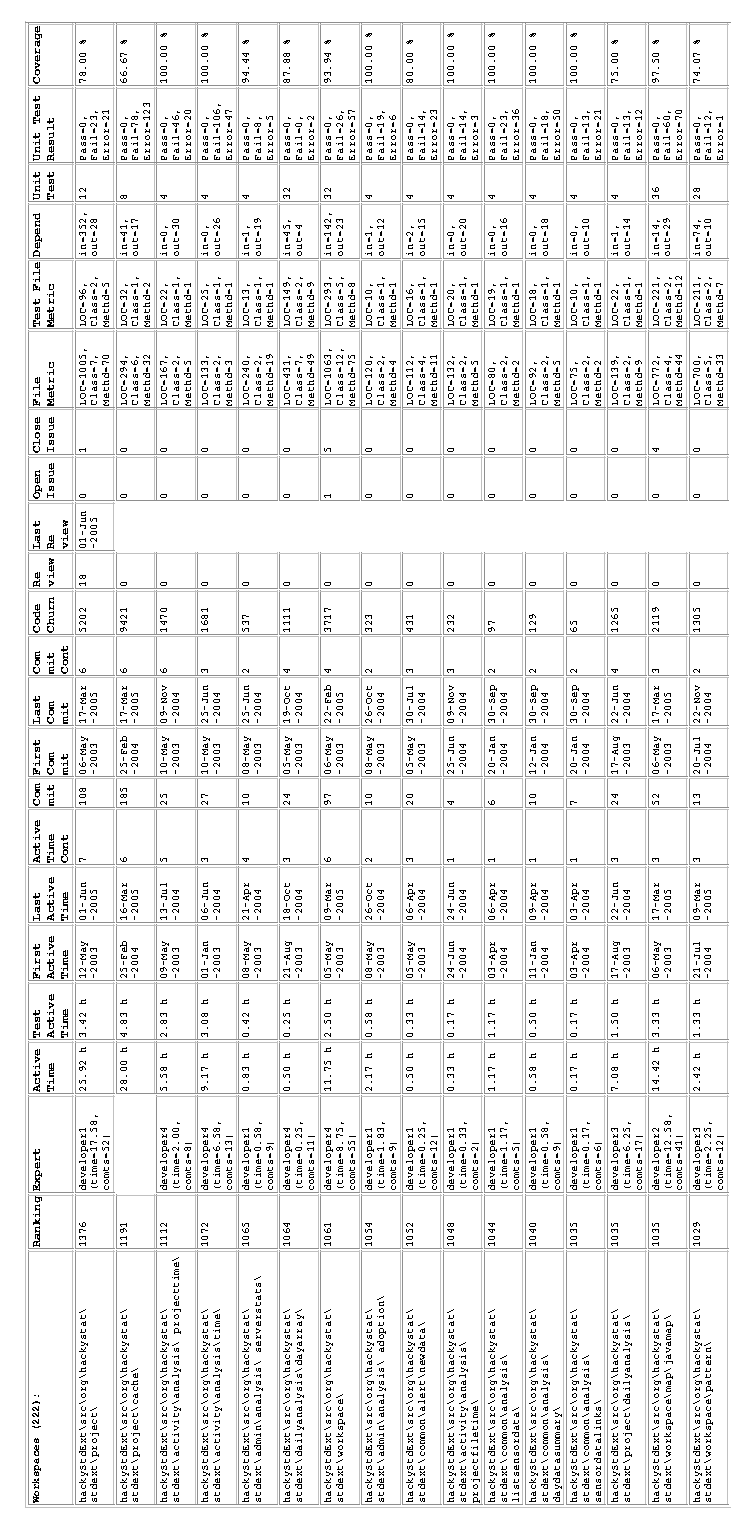
\includegraphics[totalheight=1.0\textheight]{figs/Results/17_2005-06-02-hackyStdExt-printable.eps}
  \label{fig:inspection17-hackyStdExt-ranking}
\end{figure}



